\documentclass[a4j,12pt,onecolumn,oneside,final]{jreport}

%\usepackage{gthesis}
\usepackage{gthesis_myown}

\usepackage{amsmath,amsthm,amssymb,ascmac}
\usepackage{fancybox}
\usepackage{slashbox}
%\usepackage[dviout]{color,graphics}
\usepackage{graphicx}
\usepackage{color}
\usepackage{psfrag}
%\usepackage{upgreek}
\usepackage{bm}
\usepackage{wrapfig}
\usepackage{comment}
\usepackage{url}
\usepackage{here}

%%%%%%%%%%%%%%%%%%%%%%%%%%%%%%%%%%%%%%%%%%%%%%%%%%%%%%%%%%%%%%%%
% put local tex-macros in this file %

%%%%%%%%%%%%%%%%%%%%%%%%%%%%%
%色設定
%%%%%%%%%%%%%%%%%%%%%%%%%%%%%
\definecolor{Black}{rgb}{0.0,0.0,0.0}
\definecolor{Red}{rgb}{0.9,0.0,0.1}
\definecolor{Blue}{rgb}{0.1,0.1,0.5}
\definecolor{Green}{rgb}{0.1,0.4,0.1}
\definecolor{Gray}{rgb}{0.75,0.85,0.9} % Fuji-iro
\definecolor{Shade}{rgb}{0.1,0.1,0.4}

%%%%%%%%%%%%%%%%%%%%%%%%%%%%%%%%%%%%%%%%%%%%%%%%%%%%%%%%%%%%%%%%
\年度{平成29年度}
%\提出年月{平成29年7月}
\提出年月{平成30年2月}

\題名{離散値特徴量や特異な嗜好ケースを\\考慮したコピュラを用いた推薦システム}
\梗概題名{離散値特徴量や特異な嗜好ケースを\\考慮したコピュラを用いた推薦システム}
%\題名{楽に卒業する方法に関する基礎的研究\\
%			--- そもそもそれは可能か? ---}
%\梗概題名{楽に卒業する方法に関する基礎的研究\\
%			--- そもそもそれは可能か? ---}

\指導教員名A{宮崎純}
\職名A{教授}

\指導教員名B{}
\職名B{}

%\所属学科{電気電子工学科}{}
\所属学科{情報工学科}{}
\学籍番号{14\_00368}
\氏名{朝日 諒}

\内容梗概{本研究では,コピュラを用いた既存の推薦システムの問題点を改善することで,ユーザのもつより複雑な嗜好を汲み取れるような推薦システムの構築を目指す.\par
情報推薦システムは,膨大な情報の中からユーザの嗜好にあった情報を提示するシステムである.
情報推薦システムの代表的アルゴリズムの一つであるコンテンツベースフィルタリングでは,ユーザが好むアイテムをから嗜好モデルを構築し,それに基づいて推薦を行う.\par
コンテンツベースフィルタリングで既存の推薦システムの一つに,コピュラという確率モデルを用いて嗜好モデルを構築するものがある.これは,ユーザが関心を示したアイテムを教師データとして嗜好モデルを構築するものであり,機械学習手法よりも学習結果の分析が容易であるというメリットをもつ.
しかし,このシステムの問題点として特徴量の分布が正規分布であると仮定している点,離散値の特徴量が扱えない点,特異な特徴量分布に対応できない点,などがある.\par
本論文では,これらの問題点に対し,カーネル密度推定や,ノイズを考慮した関心度式や,許容範囲フィルターを用いた手法などを組み合わせた手法を提案する.
評価実験の結果,既存の手法で用いられたデータセットでは,提案手法が既存手法と同等の結果を示し,離散値特徴量を追加した新たなデータセットでは,通常のケースと,アイテムが2値の離散値をとる特徴量をもつ場合や特徴量の分布が前述の特異な分布になるような場合を含めて,提案手法が有意水準1\%以下で既存手法よりも結果が良いことが確認できた.
}


\begin{document}
% ----------------------------------------------------------------------
% 表紙
\maketitle
% ----------------------------------------------------------------------
% 目次
\setcounter{page}{1}
\renewcommand{\thepage}{\roman{page}}
\setcounter{tocdepth}{1}
\tableofcontents
\clearpage
% ----------------------------------------------------------------------
% 内容
\setcounter{page}{1}
\renewcommand{\thepage}{\arabic{page}}
%\chapter{Introduction}
\chapter{序論}
\hspace{1em}近年,インターネットが普及しweb技術が進化することで,日々大量の情報が発信されている.
一方で,大量の情報の中から人々が自らにとって有益な情報を選択することは困難になっている.
このような問題を解決するために,ユーザの嗜好を汲み取りユーザ自身に適したアイテムを推薦するための情報推薦技術が研究され,注目を集めている.\par
情報推薦の代表的なアルゴリズムには,協調フィルタリング\cite{user-based-collaborative-filtering}\cite{item-based-collaborative-filtering}とコンテンツベースフィルタリング\cite{content-based-filtering}がある.
前者はユーザの評価履歴から求めたユーザ同士の類似度を用いて推薦を行うもので,後者はアイテムが持つ特徴量とユーザの嗜好情報から推薦を行うものである.
後者は特徴量ベースで推薦を行うため,前者と比較して新しいアイテムを推薦する場合や推薦システムの利用者が少ない場合でも機能するというメリットがある.
そこで,本研究はコンテンツベースフィルタリングを用いる.\par
コンテンツベースフィルタリングには,ユーザの評価履歴を教師データとした学習ベースで嗜好モデルを構築する手法がある.
学習ベースの手法は,ユーザ自身が嗜好情報を回答することで嗜好モデルを構築するような手法と比べて,ユーザ自身が把握しきれないような嗜好を汲み取れたり,ユーザへの負担が小さいというメリットがあるため,本研究では学習ベースのコンテンツベースフィルタリングを扱う.\par
学習手法には,機械学習手法\cite{svm}\cite{neural-network}や確率モデル\cite{Suzuki}を用いるものがある.機械学習手法には学習結果の解釈が容易でないという問題が存在するのに対して,情報推薦分野においては学習結果を解釈し,そこから新たな知見を得ることには大きな意味がある.\par
そこで鈴木ら\cite{Suzuki}は,結果の解釈が容易である確率モデルのコピュラを用いた学習手法を提案した.
鈴木らのシステムは,コピュラに特徴量の累積分布を入力することで特徴量を統合するものである.
また,鈴木らは特徴量毎にユーザが持つ関心度が異なることに着目している.
鈴木らのシステムはこの関心度とコピュラに基づいて推薦を行うため,高い精度で嗜好モデルを構築できる.\par
しかし,鈴木らのシステムにはいくつかの問題点がある.
第一に特徴量の分布モデルに正規分布を仮定しているため,実際の特徴量の分布が多峰の分布の場合に推薦精度が落ちる可能性がある.
第二に離散値の特徴量を扱えない点がある.鈴木らのシステムは特徴量の累積分布を利用するが,特徴量が離散値の場合,累積分布を定義できないため,離散値の特等量が扱えない.
第三に特異な分布,例えば特徴量値の範囲にこだわりをもつような場合,その特徴量の分布を正しく扱えないという問題がある.
鈴木らのシステムでは,特徴量の累積分布をコピュラに入力したスコア値が累積分布の単調増加になることを利用して,スコア値の高いものを優先的に推薦する.
しかし,特徴量は,特徴を数値化したものなので,その数値が高ければ良いとは限らない.よって,特徴量の数値にこだわりを持つケース,例えば高低の両端に関心をもつが,それ以外の区間には関心をもたないケースや,逆に両端ではなく,ある特定の区間に関心をもつようなケースの場合,その特徴量分布を適切に扱うことできない問題が生じる.\par
こういった問題に対処するこで,ユーザのより複雑な嗜好を汲み取れるような推薦システムの構築が期待できる.
よって,本研究では特徴量の分布モデルにカーネル密度推定を採用し,
特異な分布をもつ特徴量に対しては,特徴量のスコア値から,ユーザが強い嗜好を示す範囲を抽出するフィルターを定義し,これを用いてより複雑な嗜好を汲み取れるような推薦手法を提案する.
%unfinished
さらに評価実験により提案手法が有効であることを示す.

\chapter{基本的事項}
\section{情報推薦システム}
情報推薦システムとは,ユーザの過去の行動履歴からユーザの嗜好を汲み取り,ユーザにとって有用と思われる情報や商品などを提示するシステムである.
推薦対象の商品や情報などをアイテムと呼ぶ.動画配信サービスなどで目にすることが多い「あなたにおすすめの動画」と提示されるリストは,情報推薦システムの出力の1例である.このようなシステムに用いられるアルゴリズムは,協調フィルタリング\cite{user-based-collaborative-filtering}\cite{item-based-collaborative-filtering}とコンテンツベースフィルタリング\cite{content-based-filtering}に大別される.
\subsection{代表的な手法}
\subsubsection{協調フィルタリング}
  協調フィルタリングは推薦対象ユーザがアイテムにつけた評価値を利用して, 推薦対象ユーザまたはアイテムと似た要素からなる近傍を特定する.その後, 近傍を利用してアイテムを推薦する.\cite{rec_text}\par
\begin{comment}
大規模なサービスで用いられることの多いアイテムベースフィルタリングについて紹介する.\par
\end{comment}
表\ref{tab:user-table} のように各ユーザが各アイテムに評価値を与えていたとき, ユーザ1のアイテム5の評価値を協調フィルタリングを用いて予測することを考える.
協調フィルタリングは,近傍形成と評価値予測の方法によりユーザベースの手法\cite{user-based-collaborative-filtering}とアイテムベースの手法\cite{item-based-collaborative-filtering}に大別される.
近傍とはある要素に似たものを指す.\par
ユーザベースの場合,ユーザ間の類似度を算出し,推薦対象のユーザとの類似度が高いユーザから形成した近傍の各ユーザについて,式\eqref{eq:user_base}のように推薦対象アイテムの評価値と推薦対象ユーザとの類似度の重みつけ和により,評価値を予測する.
近傍形成にはユーザ$a$とユーザ$b$の類似度にピアソンの相関係数(式\eqref{eq:piason})を用いて,推薦対象ユーザと正の相関をもつユーザから形成する方法がある.
\\
\begin{equation}
\label{eq:piason}
sim_u(a,b)=\frac{\sum_{p\in P}^{}{(r_{a,p}-\overline{r_a})(r_{b,p}-\overline{r_b}})}{\sqrt{\sum_{p\in P}^{}{(r_{a,p}-\overline{r_a})^2}} \sqrt{\sum_{p\in P}^{}{(r_{b,p}-\overline{r_b})^2}}}
\end{equation}
$\overline{r_a}$はユーザ$a$の評価値の平均を表し,Pはアイテム集合である.
%sim_{u}=\frac{\sum_{p}^{n}{(r_{a,p}-r_a)(r_{b,p}-r_b)}}{\sqrt{\sum_{p\inP}{(r{a,p}-r_{a})^2}}\sqrt{\sum_{p}^{n}{(r_{b,p}-r_b)^2}}}
ユーザ1との相関係数はユーザ2が0.85,ユーザ3が070,ユーザ4が0.00,ユーザ5が-0.79であるため,ユーザ1の近傍ユーザはユーザ2とユーザ3である.\\
次に,この近傍ユーザ2と3の評価履歴からユーザ1のアイテム5の予測評価値$pred_u(1,5)$を式\eqref{eq:user_base}のようにして求める.
\begin{equation}
  \label{eq:user_base}
  pred_u(a,p)=\overline{r_a}+\frac{\sum_{b\in N_u}{sim_u(a,b)(r_{b,p}-\overline{r_b})}}{\sum_{b\in N_u}{sim_u(a,b)}}
\end{equation}
$N_u$は推薦対象ユーザの近傍ユーザの集合である.よってユーザ1のアイテム5の予測評価値は$4+\frac{1}{(0.85+0.7)}(0.85(3-2.4)+0.7(5-3.8))=4.87$となる

\begin{table}[ht]
 \caption{ユーザの評価値行列}
 \label{tab:user-table}
 \begin{center}
  \begin{tabular}{|lccccc|} \hline
    & アイテム1 & アイテム2 & アイテム3 & アイテム4 & アイテム5\\ \hline
    ユーザ1	& 5 & 3 & 4 & 4 & ?\\
    ユーザ2	& 3 & 1 & 2 & 3 & 3 \\
    ユーザ3	& 4 & 3 & 4 & 3 & 5\\
    ユーザ4 & 3 & 3 & 1 & 5 & 4\\
    ユーザ5 & 1 & 5 & 5 & 2 & 1\\ \hline
  \end{tabular}
 \end{center}
\end{table}
アイテムベースの場合,アイテム間で類似度を算出し,推薦対象アイテムの類似度が高いものから近傍を形成する.
アイテム間の類似度には式\eqref{eq:cos}のような,アイテムベクトル間のコサイン類似度などが用いられる.
\begin{equation}
    \label{eq:cos}
    sim_i( \vec{a}, \vec{b}) = \frac{  \vec{a} \cdot \vec{b}}{|\vec{a}| \times |\vec{b}|}
\end{equation}

\begin{comment}
ユーザ$u$の未評価のアイテム$p$に対する評価値は, 以下のアイテム$p$とユーザが評価済みのアイテム$i$との類似度の重み付け和の式$pred_i(u, p)$で予測できる.
$r_{u,i}$はユーザ$u$のアイテム$i$についての評価値である.
\begin{equation}
    \label{eq:itembase}
    pred_i(u, p) = \frac{\sum_{i\in {N_i}}{sim_i(p, i)r_{u,i}}}{\sum_{i\in N_i}{sim_i(p, i)}}
\end{equation}
\end{comment}
近傍形成後は,ユーザベースと同様に近傍$N_{i}$を対象に式\eqref{eq:itembase}のようにして,推薦対象アイテムの近傍$N_{i}$の各アイテムについて推薦対象ユーザによる評価値と推薦対象アイテムとの類似度の重みつけ和により未評価アイテムの予測評価値$pred_i(1,5)$を算出する.
\begin{equation}
    \label{eq:itembase}
    pred_i(a, p) = \frac{\sum_{b\in N_i}{sim(b,p)r_{a,b}}}{\sum_{b \in N_i}{sim(b,p)}}
\end{equation}\par
実際には, 全ての未評価アイテムの評価値を計算し, 予測された評価値の高い順番にアイテムを提示することで推薦を行う.
このように協調フィルタリングではユーザがつけた評価値のみを用いて推薦を行うため, 推薦対象アイテムについてのドメイン知識は必要ない.
また, 他のユーザの評価値を利用するため, 推薦対象ユーザにとって意外性のあるアイテムの推薦を行うことが可能となる.
しかし, 大規模なユーザ数とアイテムへの評価履歴がない場合は有効な推薦を行うことができず, このような問題はコールドスタート問題として知られている.

\subsubsection{コンテンツベースフィルタリング}
コンテンツベースフィルタリングは, アイテムが持つ性質やユーザ個人の好みを利用して推薦を行う手法である.
ユーザの好みを表す情報はユーザプロファイルとよばれる.

アイテムが持つ性質は推薦システム内では特徴パラメータとして数値で表される\cite{recOku}. アイテムの性質に応じて, 以下のような型で表現される.
\begin{itemize}
\item {\bf 連続値型}\par
   [0, 1]のような,連続値により表現できる.
    \par
    例: 価格や駅から店までの距離など
\item {\bf 二値型}\par
    二値\{0, 1\}で,ある属性を満たすかどうか表現する.
    \par
    例: 「期間限定」や「特典あり」など
\item {\bf カテゴリ型}\par
    三次元以上のパラメータを持ち, 該当する子パラメータのみ1とし, それ以外を0として表現する.
    \par
    例: 色\{ 青(1, 0, 0)赤(0, 1, 0), 黄(0, 0, 1) \}
\end{itemize}
コンテンツベースフィルタリングでは各特徴パラメータを入力として, ユーザプロファイルを用いてスコアを算出しランキング付けを行う.
スコアの算出方法は, ユーザプロファイルの形態によるが, 各特徴パラメータの重み付け和や, ユーザが好むアイテムとの類似度を計算することで算出できる.

コンテンツベースフィルタリングを用いる場合,
アイテムがどのような特徴パラメータを持っているかをシステムが知っている必要があるが,
協調フィルタリングと異なり他のユーザに依存しないため, 推薦システムの利用者が少数の場合でも推薦を行うことができる.
\subsection{評価指標}
推薦システムの性能を評価するための尺度について述べる.
推薦アイテムのうち, 正しく推薦されたアイテムを適合アイテム, そうでないものを不適合アイテムと呼ぶ.
$P@k$は推薦結果上位$k$件のうち, 適合アイテムが占める割合を示す指標. $k$件中に含まれる適合アイテムの数を$h$とすると, $P@k$は以下の式で表される.
\begin{equation}
    \label{eq:pr}
    P@k = \frac{h}{k}
\end{equation}
$nDCG@k$は, 上位$k$件の推薦結果のランキング付けの妥当性を示す指標である.
推薦結果の上位に適合度が高いアイテムが多いほど値が大きくなる指標$DCG@k$を, $DCG@k$の理想値$iDCG@k$で割って正規化した値が$nDCG@k$である.
$iDCG$は推薦結果のアイテムを適合度順にソートしたときの$DCG$を計算することで求めることができる.
 \begin{equation}
   \centering
   \label{eq:dcg}
   \mathrm{DCG}@k = \sum_{i=1}^k\frac{2^{rel_i}-1}{\log_2(i+1)}
 \end{equation}
 \begin{equation}
   \centering
   \label{eq:nDCG}
   \mathrm{nDCG}@k = \frac{\mathrm{DCG}@k}{\mathrm{iDCG}@k}
 \end{equation}
 ここで, $rel_i$は上位$i$番目アイテムの適合度である. 適合ならば1, 不適合ならば0で表現される.

 再現率$Recall_k$は推薦結果の網羅性を示す指標である. 上位$k$件中に含まれる適合アイテムを$h$, 全適合アイテムの数を$a$とすると,
 上位$k$件を取得した際の$Recall_k$は以下の式で表される.
\begin{equation}
    \label{eq:recall}
	Recall_{k} = \frac{h}{a}
\end{equation}

 iP@$i$は, 再現率が$i$の時点での推薦精度を示しており, 再現率が$i$以上における精度の最大値で表される.
 \begin{equation}
   \centering
   \label{eq:ip}
   \mathrm{iP}@i = \max_{k} \{ P@k | Recall_k \geq i \}
 \end{equation}

\newpage
\section{コピュラ}
コピュラとは,多次元の確率変数ベクトルがあるとき1次元の各確率変数の累積分布関数を入力に,多次元の同時分布を出力とする関数のことである.
\subsection{定義と基本的な性質}
$k$次元の確率変数ベクトル$X = (x_1,x_2,...,x_k)$を考える.
それぞれの累積分布関数を$cdf_k(x) = prb[X_k \leq x]$とすると,
確率変数ベクトル$X$を以下のように$k$次元単位立方空間$[0,1]^k$に写像できる.
\begin{align*}
    U = (u_1,u_2,...,u_k)
      = (cdf_1(x_1),cdf_2(x_2),...,cdf_k(x_k))
\end{align*}
このとき$k$次元同時累積分布$cdf(x_1, x_2, ..., x_n)$はある関数$C$を用いて,
\begin{align*}
  \begin{split}
  cdf(x_1, x_2, ..., x_n) &= C(cdf_1(x_1),cdf_2(x_2),...,cdf_k(x_k)) \\
  &= C(U)
  \end{split}
\end{align*}
と表せることがスクラーの定理 \cite{sklar}で知られている. この関数$C$がコピュラであり, 周辺分布間の依存関係を表す.
同時分布を構築する際, 各周辺分布のパラメータとコピュラのパラメータは個別に推定することができるため,
柔軟なモデリングが行うことができ, モデルの解釈も容易となる.\par
以下にコピュラが持つ性質を示す.
\par

\begin{itemize}
 \item
   $C(u_1,u_2,...,u_k)$は単調増加関数である.
 \item
    $Uの$要素のうち, ある一つの要素$u_i(i=1,...,k)$以外の要素が全て1ならば, $C$の値は$u_i$と一致する.
    すなわち,
   \begin{center}
   $C(1,...,1,u_i,1,...,1) = u_i$
   \end{center}
 \item
    $U$の要素のうち, 少なくとも一つの要素が0ならば, $C$の値は0となる.
    すなわち,
   \begin{center}
   $C(u_1,...,u_{i-1},0,u_{i+1},...,u_k) = 0$
   \end{center}
\end{itemize}
\par
\subsection{代表的なコピュラ}
コピュラのモデルには様々なものがあり,分布の特性に応じたモデルを選択するのが望ましい.
代表的なモデルとして式(\ref{eq:gumbel})$\sim$式(\ref{eq:clayton})のようなものがある.
$\theta$は依存関係の度合いを表すパラメータであり,$\theta$が大きいほど変数間の依存関係が強いことを意味する.
\begin{itemize}
 \item {\bf $Gumbel$コピュラ}
   \par
$C_{Gubmel}$は$u_i$が1付近で相関関係が高くなる.
    \begin{equation}
    \label{eq:gumbel}
     \centering
    C_{Gumbel}(U) = \exp(-(\sum_{i=1}^{k}(-log(u_i))^{\theta})^{\frac{1}{\theta}})
\end{equation}
\item {\bf $Frank$コピュラ}
\par$C_{Frank}$は$u_i$が0.5付近で相関関係が高くなる.
\begin{equation}
    \label{eq:frank}
    \centering
    C_{Frank}(U) = \frac{1}{\theta}log(1 + \frac{\prod_{i=1}^{k}(\exp(-\theta\ u_i) - 1)}{\exp((-\theta)-1)^{k-1}})
\end{equation}

 \item {\bf $Clayton$コピュラ}
\par$C_{Clayton}$は$u_i$が0付近で相関関係が高くなる.
\begin{equation}
    \label{eq:clayton}
    \centering
    C_{Clayton}(U) = (1 + \theta(\sum_{i=1}^{k}\frac{1}{\theta}(u_i^{-\theta} - 1)))^{\frac{-1}{\theta}}
\end{equation}
\end{itemize}

\section{カーネル密度推定}
カーネル密度推定\cite{Silverman}は,確率変数の確率密度関数を推定するノンパラメトリック手法の一つである.
$x_1,x_2,..x_n$を確率密度関数$pdf$をもつ独立同時分布からの標本とする.カーネル関数$K$,バンド幅$h$のカーネル密度推定量$\hat{pdf}$は式(\ref{eq:kde})である.
\begin{equation}
\label{eq:kde}
\hat{pdf_{h}}(x)=\frac{1}{nh}\sum_{i=1}^n K(\frac{x-x_i}{h})
\end{equation}
\label{sbsc:related_bw}
%カーネル密度推定の推定にはバンド幅$h$の影響を考慮する必要がある.
バンド幅$h$の選択は,カーネル密度推定の結果に影響する.
バンド幅に採用される値の中で,代表的なものには以下の$h_{1}$,$h_{2}$がある.\cite{Scott}\cite{Silverman}
\begin{equation*}
\label{eq:scott}
h_{1}=\left(\frac{1}{n}{\sigma}^5\right)^{\frac{1}{5}}
\end{equation*}

\begin{equation*}
\label{eq:silverman}
h_{2}=\left(\frac{4{\sigma}^5}{3n}\right)^\frac{1}{5}
\end{equation*}

\chapter{関連研究}
\section{コピュラによる適合度統合}
情報検索の分野では,複数の検索モデルで算出された適合度を統合することによって
検索精度を向上させる研究がなされてきた\cite{IR-1}\cite{IR-2}\cite{IR-3}.
Eickhoffら\cite{copulaInf}はコピュラを適合度統合に応用し,式(\ref{eq:eickhoff})を適合度統合式として提案した.
\begin{equation}
  \label{eq:eickhoff}
     \centering
  C_{prod}(U_{rel}) = C(U_{rel}) \prod_{i=1}^n u_{rel,i}
\end{equation}
$U_{rel}$は正解文書の適合度の累積分布の$n$次元ベクトルである.
各適合度の尤度の積とコピュラを掛け合わせた式(\ref{eq:eickhoff})は評価実験を行った結果, いくつかのデータセットで統合式(\ref{eq:eickhoff})が線形結合よりも有効であることを示した.
また, 様々なコピュラを用いて比較を行った結果, 情報検索のタスクにおいては$C_{Gumbel}$を用いることが適切であることを示した\cite{copulaEickhoff}.
\section{混合コピュラ}
Komatsudaら\cite{Komatsuda}は単一のコピュラでは多峰的な同時分布を表現できないことを指摘し,
複数のコピュラの重み付け和で同時分布を表現する混合コピュラを用いた統合式(\ref{eq:c-mix})を提案した.
\begin{comment}
混合コピュラを構築する手順を以下に示す.
\begin{enumerate}
\item 適合文書のクラスタリングを行う.
\item クラスタごとに周辺分布, コピュラのパラメータ推定を行う.
\item 各クラスタのコピュラを足し合わせ混合コピュラを算出する.
\end{enumerate}
\end{comment}
    以下に混合コピュラの式を示す.
    \begin{equation}
        \label{eq:c-mix}
        \centering
        C_{mix}(U_{rel})= \sum_{c=1}^{k} p_{c}C_{c}(U_{rel, c})
    \end{equation}
    ここで, $k$は文書集合のクラスタ数, $p_c$はクラスタ毎の重みで, $c$番目のクラスタに属する適合文書の割合である.
  Komatsudaらは式 (\ref{eq:c-mix}) に加え, Eickhoffらの式(\ref{eq:eickhoff}) を混合コピュラ用に拡張した式
\begin{equation}
     \label{eq:c-mix-prod}
     \centering
      C_{mix-prod}(U)= C_{mix}(U_{rel})\prod_{i=1}^n \sum_{c=1}^{k} p_{c}u_{rel,c, i}
\end{equation}
を適合度統合式として提案した. $u_{rel,c, i}$は$c$番目のクラスタに属する適合文書のi番目の適合度の累積分布を表す.
評価実験の結果, これらの統合式はEickhoffらの式よりも精度が高く, $C_{mix}$よりも$C_{mix-prod}$の方が精度が高いことが示された.

\section{関心度を考慮した特徴量統合式}
情報検索分野での適合度統合手法を情報推薦分野に適用する場合,
適合文書を適合アイテム,各適合度をアイテムの各特徴量と読み替えることで,
コピュラによる適合度統合式を情報推薦の嗜好モデル構築に適用することができる.\par
文書の適合度はユーザに依存せず客観的に表現され,高精度検索に貢献することが検証されている統計量により定義される.
これに対して,ユーザの嗜好はユーザ依存であり,全ての特徴量を対称に扱うのは不適切である.
よって,適合度統合式を嗜好モデル構築に適用する場合,ユーザがもつ各特徴量への関心度を考慮する必要がある.\par
鈴木ら\cite{Suzuki}はKL距離\cite{kl-divergence}を用いてユーザの$i$番目の特徴量に対する関心度$Att_{i}$を式(\ref{eq:Att})のように定義した.
\begin{eqnarray}
     \label{eq:Att}
     {Att}_{i} &=& \log_{1p}(D_{\mathrm{KL}}(ALL_i\|User_i)) \nonumber \\
               &=& \log_{1p}(\int_{-\infty}^{\infty} pdf_{all}(x_{i}) \log \frac{pdf_{all}(x_{i})}{pdf_{user}(x_{i})} \; dx)
\end{eqnarray}
KL距離は分布差を示す指標であり,$D_{KL}(ALL_i\|User_i)$はユーザが関心を示したアイテムと全アイテムの分布差を表している.\par
鈴木らは関心度$Att$を用いて,関心度集合$S_{Att}$から関心度が高い特徴量のみを抽出した$S_{emp}$と,$S_{Att}$から関心度が低い特徴量を除いた$S_{rdc}$を式(\ref{eq:set_emp})と式(\ref{eq:set_rdc})のように定義した.
ここでは$S_{Att}$に関して平均と分散を推定し,それらを用いて検出した外れ値を特徴量抽出に利用している.\par
外れ値の検出に必要な平均と分散は外れ値の影響が小さい$robust$な方法\cite{robust-stat}でメジアン$Med$と$MADN$(式(\ref{eq:madn}))として推定する.
鈴木らの評価実験では$cns_a=2.5$で最高の結果を示した.

\begin{eqnarray}
    \label{eq:mad}
    \centering
    MAD(S_{Att}) &=& Med(\{|Att_i - Med(S_{Att})|\}) \\
    \label{eq:madn}
    \centering
    MADN(S_{Att}) &=& \frac{MAD(S_{Att})}{0.675}
\end{eqnarray}

\begin{equation}
\label{eq:set_emp}
 \centering
S_{emp}=\{i|Med(S_{Att})+cns_a\cdot MADN(S_{Att})\leq Att_i\}
\end{equation}

\begin{equation}
\label{eq:set_rdc}
S_{rdc}=\{i|Att_i \leq Med(S_{Att})-cns_a\cdot MADN(S_{Att})\}
\end{equation}

\begin{comment}
\begin{flalign}
\label{eq:set_emp}
 \centering
&S_{emp}=\{i|Med(S_{Att})+cns_a\cdot MADN(S_{Att})\leq Att_i\}& \\
\label{eq:set_rdc}
   \centering
&S_{rdc}=\{i|Att_i \leq Med(S_{Att})-cns_a\cdot MADN(S_{Att})\}&
\end{flalign}
\end{comment}
鈴木らは,$S_{rdc}$と$S_{emp}$と,小松田らの混合コピュラ式(\ref{eq:c-mix-prod})から関心度を反映させた統合式(\ref{eq:kl-emp-prod})を提案した.
統合式$C_{kl-emp-rod}$は特定の評価指標について既存の統合式と比較して最高の結果を示した.

\begin{equation}
    \label{eq:kl-emp}
    \centering
    C_{kl-emp}(U_{rdc}) =  C_{mix}(U_{rdc}) \prod_{i \in S_{emp}} \sum_{c=1}^{k} p_{c}u_{rel,c, i}
\end{equation}
\begin{equation}
    \label{eq:kl-emp-prod}
    \centering
    C_{kl-emp-prod}(U_{rdc}) = \begin{cases} C_{mix-prod}(U_{rdc}) & \text{if}\; S_{emp} =	 \emptyset\\ C_{kl-emp}(U_{rdc}) & \text{otherwise}\;   \end{cases}
\end{equation}

\chapter{提案手法}
\label{ch:proposal}
\begin{figure}[H]
  \begin{center}
    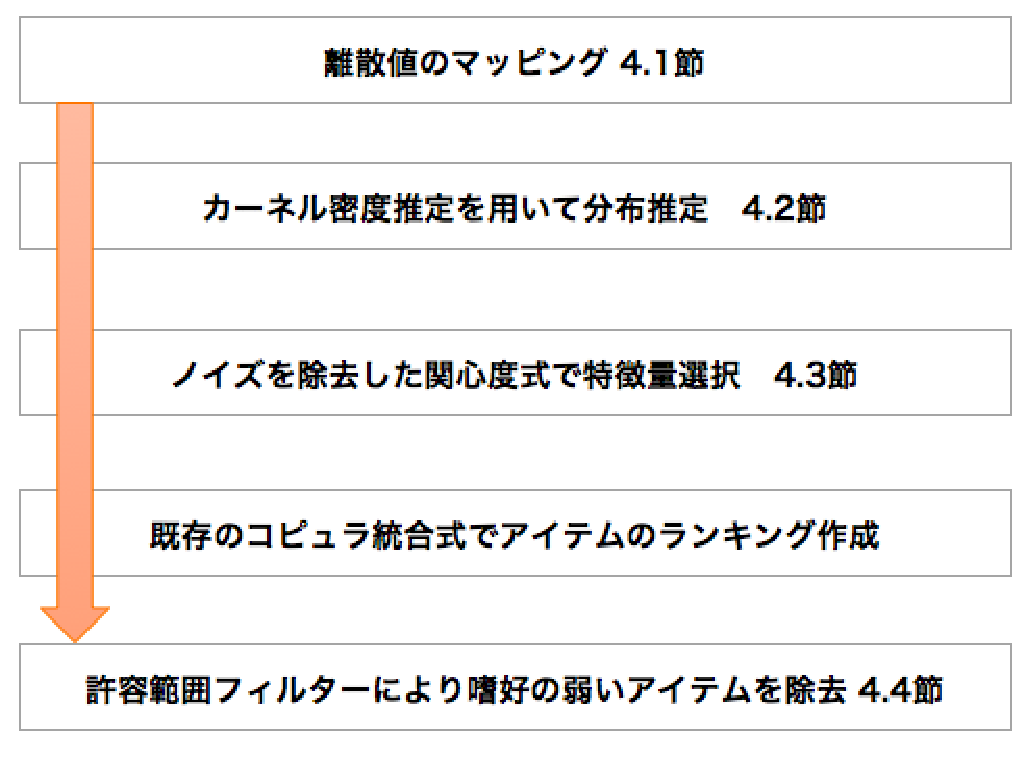
\includegraphics[width=5in]{source/proposal.eps}
  \vspace{1mm}
  \caption{提案手法の処理チャート} %\vspace{-3mm}
  \label{fig:proposal}
  %\vspace{-0.4cm}
  \end{center} 
\end{figure}
\hspace{1em}本提案手法は以下の4つの構成から成っており,鈴木らのシステムでは扱えない離散値特徴量や特異な分布を扱うためのものである.\par
提案手法の処理チャートは図\ref{fig:proposal}である.
\begin{enumerate} 
  \item ユーザの嗜好を反映した離散値特徴量への数値マッピング (\ref{sc:mapping}節)
  \item カーネル密度推定を利用した複雑な分布への対応 (\ref{sc:mix_gaussian}節)
  \item 鈴木らの関心度式からノイズ部分を除去して,離散値特徴量へ対応 (\ref{sc:att_shr}節)
  \item 許容範囲フィルターにより,特徴量値の特定区間にこだわりをもつような特異な嗜好ケースに対応 (\ref{sbsc:tlr}節)
\end{enumerate}
\section{離散値特徴量への数値マッピング}
\label{sc:mapping}
特徴量の累積分布を求めるためには,特徴量を数直線上の実数値にマッピングする
必要がある.
特徴量の累積分布は特徴量に対して単調増加するため,
特徴量が離散値の場合,数値を離散値に割り当てる順番が累積分布の値に影響する.
この際にユーザがもつ,離散値特徴量への嗜好順を考慮すべきである.\par
例えば,喫煙可能か禁煙かを表す離散値特徴量として喫煙値というものを定義し,これに0と1の数値を割り当てる場合を考える.
ユーザが禁煙家の場合は禁煙に1,喫煙可能に0を割り当てるべきなのに対し,ユーザが喫煙家の場合は喫煙可能に1,禁煙に0を割り当てるべきである.\par
このように嗜好順を考慮したマッピングをするために人気度$ppl$を以下のように定義した.
$i$番目の特徴量の離散値$v$に対して,ユーザがもつ人気度$ppl_i(v)$は式(\ref{eq:ppl})で定義される.
\begin{comment}
  \label{eq:popular}
  &like_{User}(x)=\left\{
    \begin{array}{ll}
      1 &(User\hphantom{a}likes\hphantom{a}x) \\
    0 &(otherwise) 
\end{array}\right. & \\
  &S_{User}=\{item|like_{User}(item)==1\}& \\
\end{comment}

\begin{gather*}
  S_{ScoreUser}(i,v)=\{item|score_{i}(item)=v\}\cap S_{User} \\
  S_{ScoreAll}(i,v)=\{item|score_{i}(item)=v\}\cap S_{All} \\
\end{gather*}
\begin{equation}
  \label{eq:ppl}
  ppl_i(v)=\frac{|S_{ScoreUser}(i,v)|}{|S_{ScoreAll}(i,v)|}
\end{equation}\par
$score_{i}(item)$は$item$の特徴量$i$のスコア値を返す関数,$S_{User}$はユーザが選択した$item$集合,$S_{All}$は全$item$集合であることに注意する.
$ppl_i(v)$は$i$番目の特徴量が$v$の$item$集合から,ユーザがどれだけの$item$に関心を示したかを表している.\par
この人気度$ppl$の高い離散値から降順で高い数値を割り当てることで,ユーザの嗜好を考慮して,離散値特徴量に数値を割り当てられることが期待できる.
\section{カーネル密度推定を利用した複雑な分布への対応}
\label{sc:mix_gaussian}
鈴木らのシステム\cite{Suzuki}が特徴量分布の推定に正規分布モデルを用いていたのに対し,本研究ではカーネル密度推定を用いる.
これにより,特徴量の分布が正規分布にならない場合にも対応できることが期待できる.
式(\ref{eq:kde})のパラメータであるカーネル関数式には式(\ref{eq:kernel})を
用いた.
\begin{equation}
\label{eq:kernel}
K(x)=\left\{
\begin{array}{ll}
  tophat(x) & (特徴量xが離散値) \\
  gaussian(x) & (特徴量xが連続値) \\
\end{array} \right.
\end{equation}

\begin{equation}
  \label{eq:tophat}
  tophat(x)=\left\{
  \begin{array}{ll}
    \frac{1}{2} &(-1 \leq x \leq 1) \\
    0 &(otherwise) \\
  \end{array} \right.
\end{equation}

\begin{equation}
  \label{eq:gaussian}
  gaussian(x)=
  \frac{1}{2\sqrt{\pi}\sigma}exp\left(-\frac{{(x-u)}^2}{2{\sigma}^2}\right) \\
\end{equation}

\subsection{バンド幅の決定}
カーネル密度推定式(式(\ref{eq:kde}))のパラメータであるバンド幅$h$の選択には式(\ref{eq:h})のようにカーネル関数$K(x)$の特性に合ったものを用いた.
連続値の場合,最適値の位置を探るための$S_{lct}$と\ref{sbsc:related_bw}の$h_{2}$,$h_{1}$からなる$S_{opt}$から構築した探索集合$S_{Grd}$から$GridSearch$で最適値$h_{G\_opt}$を選択する.
$S_{lct}$は$K(x)$が$gaussian(x)$で累積分布が求まるという条件と,常用対数が負であるという条件を同時に満たす要素の集合である.\\
\begin{equation}
  \label{eq:h}
  h_{opt}=\left\{
    \begin{array}{ll}
  0.1 &(K=tophat)\\
  h_{G\_opt} &(K=gaussian)
\end{array}\right.
\end{equation}

\begin{gather}
\label{eq:kde_lct}
S_{lct}=\{10^{-3},5\cdot 10^{-3},10^{-2},...,5\cdot 10^{-1}\} \\
\label{eq:kde_opt}
S_{opt}=\{silverman,scott\} \\
\label{eq:kde_search}
S_{Grd}=S_{lct}\cup S_{opt}
\end{gather}


\begin{comment}
\begin{flalign}
\label{eq:kde_lct}
&S_{lct}=\{10^{-3},5\cdot 10^{-3},10^{-2},...,5\cdot 10^{-1}\}& \\
\label{eq:kde_opt}
&S_{opt}=\{silverman,scott\}& \\
\label{eq:kde_search}
&S_{Grd}=S_{lct}\cup S_{opt}&
\end{flalign}
\end{comment}
以下に$Gridserach$の概要を載せる.
\begin{enumerate}
  \item 訓練用データ集合$S_{trn}$からこれを$k$分割した各集合$S_{Nscr\_i}$を除いた評価用集合$S_{scr\_i}$を得る.
  \item $S_{Grd}$から,未評価の要素$h$をとりだす.
  \label{itm:grd1}
  \item 式(\ref{eq:score_i_h})のようにして$S_{scored\_i}$で$h$の評価値を求める.
  \item 式(\ref{eq:score_h})のようにして全評価用集合での評価値平均を$h$の評価値とする.
  \label{itm:grd2}
\item (\ref{itm:grd1})から(\ref{itm:grd2})を全$h$に対して行い,$h$の評価値が最大となるものを$h_{G\_opt}$とする.
\end{enumerate}
\begin{eqnarray}
  \label{eq:trn_data}
  S_{scr\_i}&=&S_{trn}\backslash S_{Nsrc\_i} \\
  \label{eq:score_i_h}
  score(h,i)&=&\sum_{x\in S_{scored\_i}}\log f(x) \\
  \label{eq:score_h}
  score(h)&=&\frac{1}{k}\sum_{i=1}^k score(h,i)
\end{eqnarray}
\par
離散値の場合,カーネル関数が$tophat$なので各離散値点で$tophat$が干渉しないようなバンド幅を選択すれば推薦に必要な累積分布を得ることができる.
本研究で用いる離散値は0と1の値をとるため,バンド幅は$0.5$以下になればよい.
よって,離散値のバンド幅には,$0.5$未満で,常用対数が整数であるという条件をみたす実数の最大値である$0.1$を採用した.

\begin{comment}
Set_{int}&=&\{x|\log_{10} x \in \mathbb{Z}\land\\
         && -3 <\log_{10} x < 0\} \nonumber \\
\label{eq:kde_middle}
Set_{middle}&=&\{x| x=middle(y_i,y_{i+1})\}\\
\end{comment}

\section{ノイズを除去した関心度式}
\label{sc:att_shr}
既存の鈴木らの関心度式$Att_i$(式(\ref{eq:Att}))では積分区間が無限区間であり,スコア値の範囲である区間[0,1]以外の計算結果が含まれていた.
しかし,区間[0,1]以外の計算結果をノイズとしたとき,離散値の場合,$tophat$を用いるためノイズが0になる.
よって既存の関心度式で連続値と離散値を比較する場合,ノイズ差を考慮していない問題が生じる.
よって新たな関心度式(式(\ref{eq:new_att}))を$Att_{i\_Shr}$として提案する.
\begin{eqnarray}
     \label{eq:new_att}
     {Att}_{i\_Shr} &=& D_{\mathrm{KL}}(User_i\|ALL_i) \nonumber \\
               &=& (\int_{0}^{1} pdf_{user}(x_{i}) \log \frac{pdf_{user}(x_{i})}{pdf_{all}(x_{i})} \; dx)
 \end{eqnarray}
 \par
 式(\ref{eq:new_att})は既存の算出式$Att$の積分区間を変更し,ノイズが計算結果に含まれないようにしたものである.
 さらに$pdf_{all}(x)\leq pdf_{user}(x)$の部分をより反映させるために鈴木らが用いた$D_{\mathrm{KL}}$のベースを$All_i$から$User_i$へ変更した.区間変更に伴い,値調整のための$log_{1p}$が不要になったためこれを取り除いた.

\section{許容範囲フィルター}
\label{sbsc:tlr}
\begin{table}[H]
  \begin{center} {
    \caption{特異な分布例} \label{tbl:abnormal_role}
    \begin{tabular}{lp{25em}} 
\hline
ROLE番号 & ROLEの説明\\ \hline
ROLE7 & 駅の騒音と徒歩距離を考慮して,駅から適度な距離のホテルがよい.\\
ROLE14 & 同僚と出張で宿泊する.6,000円/人まで会社経費.ホテルはルームチャージ制のため,個人利用であれば,低価格のホテルしか利用できず,相部屋で利用する場合,高価格のホテルまで利用できる.\\
\hline
    \end{tabular}
  }
  \end{center} %\vspace{-8mm}
\end{table}
鈴木らのシステム\cite{Suzuki}はユーザの選択したアイテムを教師データとして構築したコピュラモデルから,推薦対象のアイテムの累積分布を求め,その累積分布の降順で推薦を行うものである.しかし予備調査の結果,表\ref{tbl:abnormal_role}のROLE7やROLE14のような状況において,特徴量の数値が高いがユーザが関心を示していないアイテムが上位に推薦されてしまうという問題が生じため$tlr$の提案を行う.\par
$tlr_i$は特徴量$i$と,ユーザが選択したアイテムの密度分布$pdf_{user}(x)$と,全アイテムの密度分布$pdf_{all}(x)$を考えるとき,式(\ref{eq:tlr})のように定義される.
\begin{equation}
\label{eq:tlr}
tlr_{i}=\{x | pdf_{all,i}(x) \leq pdf_{user,i}(x)\}
\end{equation}
\par
$tlr_i$は,特徴量$i$について全アイテムの$pdf$である$pdf_{all,i}$よりも,ユーザが関心を示したアイテムの$pdf$である$pdf_{user,i}$が上回るような区間であり,ユーザが特に関心を示す特徴量値の範囲を抽出するためのものである.
許容範囲フィルターを特異な分布をとる特徴量$i$の値が,$tlr_{i}$に含まれるアイテムを優先的に選択する手法として定義する.
この手法を用いれば,特定の特徴量値が特定の範囲にあるアイテムに強い嗜好を示すようなケースに対応できることが期待できる.\par
しかし,この許容範囲フィルターを有効にする特徴量をどのようにして選択するかという問題がある.
許容範囲フィルターを有効にする特徴量が多いほど,アイテムが推薦対象から外される可能性が高くなりフィルターが有効に機能しにくくなる.\par
よって,特異な分布をとる特徴量を含むできるだけ小さい特徴量集合で,フィルターを有効にするのが望ましい.
特異な分布をとる特徴量の場合,ユーザはその特徴量に強い関心をもっていることが想定される.
よって,鈴木らの手法を用いて重要次元$S_{emp}$(式(\ref{eq:set_emp}))を抽出して,$S_{emp}$でフィルターを有効にするという手法が候補に上がる.
しかし,関心度が一部の特徴量で拮抗しているため重要な特徴量が外れ値として検出できないような場合に,特定の特徴量が特異な分布をとるにもかかわらずフィルターが有効にならないというケースを考慮して,フィルターを有効にする特徴量集合$S_{fitered}$を(式(\ref{eq:S_filtered}))のように定義する.

\begin{equation}
\label{eq:S_filtered}
S_{filtered}=\left\{
  \begin{array}{ll}
    S_{sorted}(n) &(S_{emp}=\phi)\\
    S_{emp} &(otherwise)\\
  \end{array}\right.
\end{equation}
\par
(式(\ref{eq:S_filtered}))は重要次元$S_{emp}$が要素をもつ場合は$S_{emp}$の特徴量でフィルターを有効にし,$S_{emp}$が空の場合は鈴木らの関心度式で算出した関心度の降順で$n$番目までの特徴量からなる集合$S_{soreted}(n)$の特徴量でフィルターを有効にすることを意味する.
$n$には,評価実験でU字型の分布が確認できた全特徴量を抽出できる整数のうち,最小の値である$n=2$を用いた.\par
この$S_{filtered}$の各特徴量$i$の値が$tlr_i$に含まれるという条件を満たすようなアイテムを優先的に推薦することで,特異な分布をとらない特徴量による影響を抑えつつ許容範囲フィルターを用いて適切な推薦ができることが期待できる.

\chapter{評価実験}
\hspace{1em}提案手法が,既存の手法では扱えないような問題ケースで有効に機能するかを検証するために,離散値の特徴量を含む新たなデータセットを用いて評価実験を行う.また,問題ケースに限定せず既存の手法で扱えた通常のケースでも有効に機能するかを検証するために,旧データセットを用いた評価実験も行う.
\section{実験条件}
データセットには,鈴木らが用いた旧データセットと旧データセットに変更を加えた新データセットを用いた.
旧データセットは連続値のみを特徴量にもつデータセットである.これは,楽天トラベルのホテルデータのうち, 東京 23 区内のホテル 245 件を対象としている.
各ホテルは, 価格, サービスレビュー, 施設レビュー, 部屋レビュー, 立地レビュー, 風呂レビュー, 食事レビュー, 最寄り駅からの直線距離の計8種類の情報を持つ.
各レビュー値は楽天トラベル利用者が評価した1-5の五段階評価の平均値で, 未評価の場合は0となる.
価格はそのホテルの全宿泊プランの価格の中央値である.
これらの値の取りうる範囲が[0, 1]になるように正規化したものを特徴量としている.\par
新データセットは,この旧データセットに9個目の新たな特徴量として喫煙値を加えたものである.
喫煙値には喫煙可と禁煙の2値を定義し,各ホテルに各離散値を$50\%$の確率で割り当てた.
\par
被験者の実人数は大学院生12人で,延べ人数が33人である.
\par
また,実験手順は下記の通りである.

\begin{enumerate}
  \item 被験者は割り振られたROLEのシナリオ下でホテルを評価する.全ROLEは表\ref{tbl:ROLE}の通りである.
  \item ホテル評価時に重視した特徴量に合計100となるように重みを割り振る.
  \item ホテル評価時の喫煙値への立場として極度に悪い,悪い,中立,良い,極度に良い,の5段階で最も近いものを選択する.
\end{enumerate}
\begin{table}[H]
  \begin{center} {
    \caption{ROLE一覧} \label{tbl:ROLE}
    \begin{tabular}{p{7em}lp{25em}} 
\hline
期待する分布 & ROLE番号 & ROLEの説明\\ \hline
特になし & ROLE1 &出張で宿泊する.会社規定のため安く済ませたい.\\ 
&ROLE2 & 友達と旅行で宿泊する.\\ 
&ROLE3 & 観光目的で宿泊する.価格は気にせず良いホテルがよい.\\ 
&ROLE4 & 恋人と宿泊する.安くて良いホテルがよい.\\ \hline
離散値で偏った分布&ROLE5 & ROLE3+被験者には数日おきに喫煙習慣がある.\\ 
&ROLE6 & ROLE4+恋人が喫煙者である.\\
&ROLE9 & ROLE1+被験者は極度の嫌煙家である.\\
&ROLE10 & ROLE2+被験者は極度の喫煙家である.\\ 
&ROLE11 & ROLE2+被験者は極度の嫌煙家である.\\ 
&ROLE12 & ROLE3+被験者は極度の喫煙家である.\\ 
&ROLE13 & ROLE4+被験者は極度の嫌煙家である.\\ \hline
特異な分布&ROLE7 & 駅の騒音と徒歩距離を考慮して,駅から適度な距離のホテルがよい.\\
&ROLE14 & 同僚と出張で宿泊する.6,000円/人まで会社経費.ホテルはルームチャージ制のため,個人利用であれば低価格のホテルしか利用できず,相部屋で利用する場合高価格のホテルまで利用できる.\\
\hline
    \end{tabular}
  }
  \end{center} %\vspace{-8mm}
\end{table}

\section{比較手法}
\begin{itemize}
 \item {\bf 嗜好回答情報を利用した重み付け線形和}
    \par
    \begin{equation}
        \label{eq:line-method}
        \centering
        LIN(X) = {\sum_{i=1}^n{w_i x_i}}
    \end{equation}
    $i$番目の特徴パラメータへの重み$w_i$値は, 対応する嗜好回答データの値をその総和である100で割ったものである.
  \item {\bf コピュラを用いた統合式}
    \par
    \begin{equation*}
      \label{eq:copula-method}
      method=C_{A,B,C}
    \end{equation*}
    \begin{equation*}
        \label{eq:marg_option}
        \centering
  A=\left\{
    \begin{array}{ll}
      'Kd' & (カーネル密度推定) \\
      'Nrm' & (正規分布) \\
    \end{array} \right.
    \end{equation*}
    \begin{equation*}
        \label{eq:attn_option}
        \centering
  B=\left\{
    \begin{array}{ll}
      'Shr' & (att=Att_{Shr}) \\
      'Inf' & (att=Att_{Inf}) \\
    \end{array} \right.
    \end{equation*}

    \begin{equation*}
        \label{eq:tl_option}
        \centering
  C=\left\{
    \begin{array}{ll}
      'Tl' & (フィルター有効) \\
      NULL & (フィルター無効) \\
    \end{array} \right.
    \end{equation*}

    鈴木らの$C_{kl-emp-prod}$(式(\ref{eq:kl-emp-prod}))に,\ref{ch:proposal}章で述べた各小手法を部分的に有効にした手法である.用いるコピュラ統合式を$method$としたとき,$method$は,$C_{A,B,C}$のように表す.フィルターを用いる場合,Cの文字列は$'Tl'$であり,フィルターを用いない場合$C$は$NULL$で空文字であることに注意する.\par
例えば,鈴木らの既存手法の場合,分布推定に正規分布を用いて,関心度式には$Att_{Inf}$を用いるため,その表記は$C_{Nrm,Inf}$である.提案手法の場合,分布推定にカーネル密度推定を用い,関心度式には$Att_{Shr}$を用い,フィルターを有効にするため,その表記は,$C_{Kd,Shr,Tl}$である.
\begin{comment}
\item $C_{KdTlShr}$.カーネル密度推定,Tolerance,Short
\item $C_{KdTlInf}$.カーネル密度推定,Tolerance,Informal
\item $C_{KdShr}$.カーネル密度推定,Short
\item $C_{KdInf}$.カーネル密度推定,Informal
\item $C_{NrmTlShr}$.正規分布,Tolerance,Short
\item $C_{NrmTlInf}$.正規分布,Tolerance,Informal
\item $C_{NrmShr}$.正規分布,Short
\item $C_{NrmInf}$.正規分布,Informal
\end{comment}
\item {\bf ランキングSVM}
    \par
    $SVM^{rank}$ \footnote{\url{https://www.cs.cornell.edu/people/tj/svm_light/svm_rank.html}} \cite{rankingSVMTool}を用いて, ランキングSVMモデルを構築する.
    コストパラメータ$C$には$SVM^{rank}$のデフォルト値である$0.01$を用い,カーネルにはRBFカーネルを用いた.
    カーネルがもつパラメータ$\gamma$には, $2^{-10}, 2^{-9}, ..., 2^{9}, 2^{10}$の候補の中から, 最も精度が高いものを用いることにした.よって,旧データセットでは$2^3$,新データセットでは,$2^4$を用いた.
\end{itemize}

\section{提案手法のパラメータ}
提案手法で用いたパラメータは以下の通りである.
\begin{itemize}
  \item コピュラモデルには,$C_{frank}$,$C_{Clayton}$,$C_{gumbel}$の中で,最も良い精度を示したものを採用した.よって,旧データセットでは,鈴木らの手法で最高の精度を示した$C_{gumbel}$を用い,新データセットでは,提案手法で最高の精度を示した$C_{frank}$を用いた.
\item クラスタ数は,1$\sim$5に変化させた時に最も良い精度を示したものを採用した.よって,旧データセットでは,鈴木らの手法で最高の精度を示した5を用い,新データセットでは,提案手法で,最高の精度を示した2を用いた.
\item 特徴量選択時の正定数$cns_a$には,$1.0\sim3.5$まで0.5刻みで変化させた時に最高の精度を示したものを採用した.よって,旧データセットでは,鈴木らのシステムで最高の精度を示した2.5を採用し,新データセットでは,提案手法で最高の精度を示した1.5を採用した.
\item $GridSearch$(式(\ref{eq:score_h}))のパラメータ$k$には,使用したライブラリのデフォルト値である3を採用した.
\end{itemize}
コピュラモデル,クラスタ数,正定数については,新データセットでの候補比較の結果を付録\ref{ch:appendix}に掲載した.
\section{実験結果}
\subsection{ROLE別離散値選択}
評価実験で用いたROLE(表\ref{tbl:ROLE})に対して,ROLE別の被験者数,禁煙アイテム選択率は表\ref{tbl:RoleUserSmoke}の通りである.
禁煙アイテム選択率は被験者が関心を示したアイテムに占める,喫煙値が禁煙となるアイテムの割合と定義しているので,禁煙アイテム選択率が高いほど禁煙のアイテムをより優先的に選択したことを意味する.禁煙アイテムを優先的に選択するケース,喫煙可能アイテムを優先的に選択するケース,アイテムの喫煙値に偏りがないケースの3つが少なくとも一つはサンプルを持つことが確認できる.
\begin{table}[t]
    \caption{ROLE別の被験者数と禁煙アイテム選択率} \label{tbl:RoleUserSmoke}
    \begin{tabular}{p{7zw}p{5em}p{5zw}l} 
\hline
想定する分布&ROLE&被験者数& 禁煙アイテム選択率 \\ \hline
なし&ROLE1&2& 0.55,0.56\\ 
&ROLE2&4& 0.52,0.55,0.70,0.99 \\ 
&ROLE3&1& 0.62 \\ 
&ROLE4&2& 0.51,0.51 \\ \hline
喫煙家または嫌煙家&ROLE5&2& 0.43,0.55 \\ 
&ROLE6&1& 0.07 \\
&ROLE9&1&0.89 \\ 
&ROLE10&1& 0.12 \\ 
&ROLE11&1& 0.9 \\ 
&ROLE12&1& 0.2 \\ 
&ROLE13&2& 1.0,1.0 \\  \hline
特異な分布&ROLE7&6& 0.48,0.53,0.57,0.65,0.66,0.96 \\ 
&ROLE14&9& $0.45,0.47,0.5,0.53,0.53,0.55,0.57,0.77,1.0$ \\ \hline
    \end{tabular}
\end{table}

\subsection{特異な分布}
評価実験では,特定の特徴量が鈴木らのシステムでは対応できないような特異な分布をとることを想定したケースを表\ref{tbl:ROLE}のROLE7,ROLE14として用いた.\par
\label{sbsc:ROLE7}
ROLE7は駅の喧騒が気にならない程度に駅から離れていて,通勤に不便にならない程度に駅から近いホテルを探すという設定である.よって距離スコアが高すぎるとユーザに選択されないことが想定される.\par
ROLE7の分布図\ref{fig:ROLE7-distance}と通常の分布であるROLE1の分布図\ref{fig:ROLE1-distance}を比較する.これらの図からは許容範囲$tlr$に関して通常の分布ではscoreの右端まで連続しているのに対して,ROLE7では右端付近で途切れているのが確認できる.
よって,これに許容範囲フィルターを適用することで,ユーザが強い嗜好を示す範囲のアイテムを優先的に選択することができるため,ROLE7の場合でも適切な選択ができることが期待できる.\par
\label{sbsc:ROLE14}
ROLE14は,6,000円付近の低価格帯と12,000円付近の高価格帯のホテルを優先的に選択させる設定であり,価格特徴量の分布が低価格帯と高価格帯で峰になるU字型の分布になることを想定したものである.\par
6,000円以下の低価格帯のホテルの場合,ホテルのレビュー値が低いというデメリットと個室利用できるというメリットがある.
一方,12,000円付近の高価格帯のホテルの場合,個室利用ができないというデメリットと,ホテルのレビュー値が高いものが多いというメリットがある.
両価格帯の中間に位置する中価格帯の場合,個室利用ができず,レビュー値も高価格帯のホテルより劣るものが多いため,選択するメリットが小さい.\par
よって,ユーザはメリットの薄い中価格帯では選択を控え,メリットとデメリットが等しく存在する両端の価格帯でホテルの選択をするため,価格特徴量の分布がU字になることが想定される.\par
ROLE14の分布(図\ref{fig:ROLE14-charge})は想定通り,U字型になっている.
U字型の分布の場合,U字の谷の部分ではユーザが選択を避けているため,全アイテムの分布よりも$pdf$が下回る傾向がある.よって,許容範囲フィルターをこの特徴量分布に適用し,U字の谷の部分を推薦対象から外すことで,ROLE14の中価格帯のアイテムを誤って推薦するというケースは避けられる.\par
U字の両峰付近のアイテムについては,鈴木らのコピュラ統合式により価格特徴量とその他のレビュー値を統合できるため,これを用いてアイテムの順位付けができる.よって許容範囲フィルターを用いれば,ROLE14のようなU字型の分布でも適切な推薦ができることが期待できる.

\begin{figure}[H]
  \begin{center}
    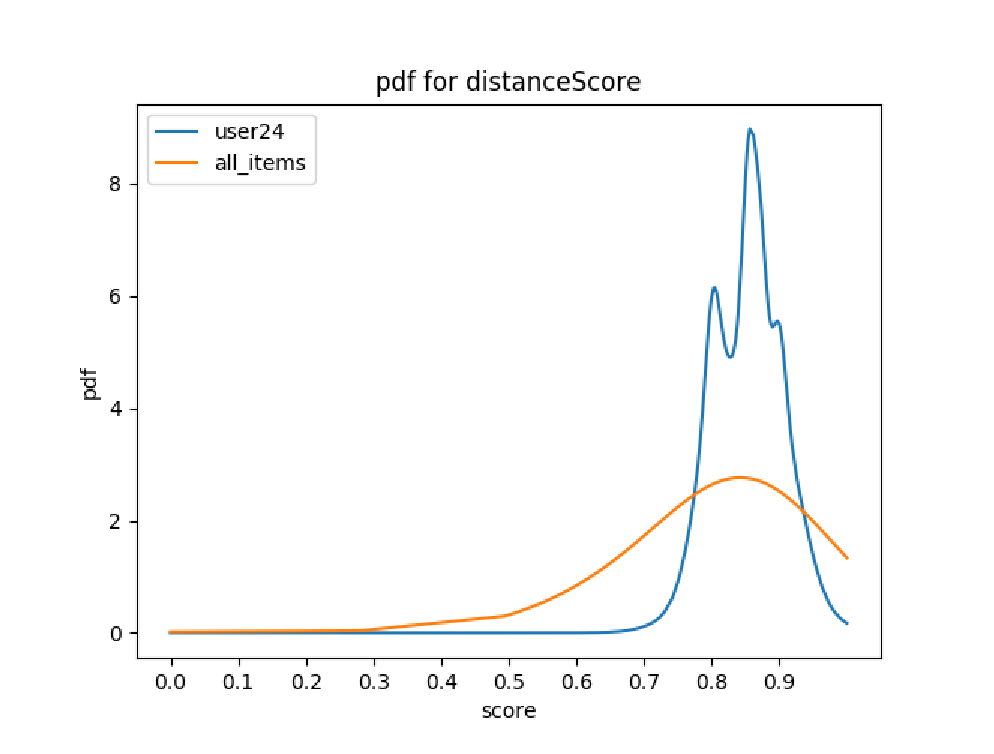
\includegraphics[width=6in]{source/ROLE7-distance.eps}
  \vspace{1mm}
  \caption{ROLE7の距離特徴量分布} %\vspace{-3mm}
  \label{fig:ROLE7-distance}
  %\vspace{-0.4cm}
  \end{center} 
\end{figure}

\begin{figure}[H]
  \begin{center}
    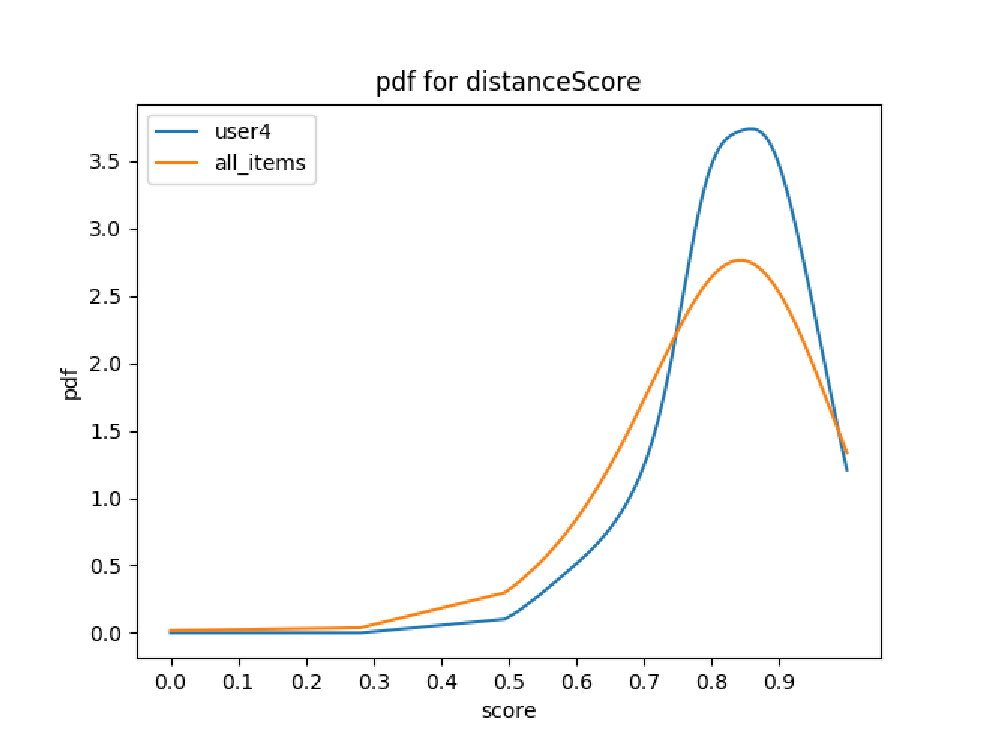
\includegraphics[width=6in]{source/ROLE1-distance.eps}
  \vspace{1mm}
  \caption{ROLE1の距離特徴量分布} %\vspace{-3mm}
  \label{fig:ROLE1-distance}
  %\vspace{-0.4cm}
  \end{center} 
\end{figure}

\begin{figure}[H]
  \begin{center}
    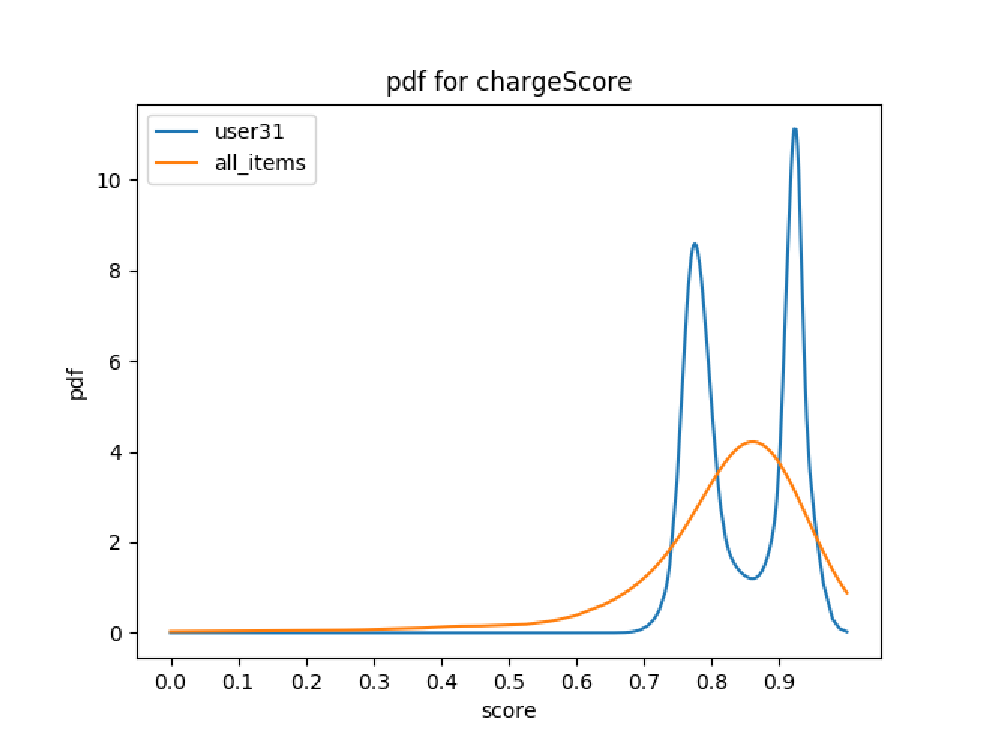
\includegraphics[width=6in]{source/ROLE14-charge.eps}
  \vspace{1mm}
  \caption{ROLE14の価格特徴量分布} %\vspace{-3mm}
  \label{fig:ROLE14-charge}
  %\vspace{-0.4cm}
  \end{center} 
\end{figure}



\begin{table*}[h]
  \caption{旧データセットでの実験結果} 
  \label{tbl:resultOld}
  \begin{center} {
\scalebox{0.9}[1]{
    \begin{tabular}{|l|l|l|ll|} \hline
      measure&$C_{Kd,Shr,Tl}$(提)&$C_{Nrm,Inf}$(既)&$LIN$&$SVM$\\ \hline
iP@0&1.0&0.995&0.98&0.991\\
iP@0.1&0.994&0.992&0.959&0.986\\
iP@0.2&0.976&0.99&0.94&0.981\\
iP@0.3&0.954&0.955&0.918&0.965\\
iP@0.4&0.92&0.934&0.884&0.958\\
iP@0.5&0.899&0.922&0.849&0.945\\
iP@0.6&0.848&0.888&0.811&0.913\\
iP@0.7&0.808&0.845&0.772&0.863\\
iP@0.8&0.755&0.756&0.709&0.814\\
iP@0.9&0.696&0.64&0.633&0.741\\
iP@1.0&0.568&0.503&0.531&0.634\\ \hline
MAiP&0.856&0.856&0.817&0.89\\ \hline
nDCG@5&0.995&0.992&0.96&0.981\\
nDCG@10&0.987&0.987&0.957&0.98\\
nDCG@15&0.981&0.981&0.952&0.977\\
nDCG@20&0.975&0.978&0.949&0.974\\
nDCG@30&0.967&0.972&0.942&0.969\\ \hline
P@5&0.954&0.954&0.887&0.946\\
P@10&0.888&0.9&0.862&0.923\\
P@15&0.81&0.847&0.799&0.857\\
P@20&0.764&0.775&0.732&0.794\\
P@30&0.648&0.638&0.617&0.669\\ \hline
\end{tabular}
  }
    }
  \end{center}
\end{table*}

\begin{table*}[h]
  \caption{旧データセットでの提案手法との比較におけるU検定でのp値} 
  \label{tbl:resultOldUP}
  \begin{center} {
\scalebox{0.9}[1]{
\begin{tabular}{|l|l|ll|} \hline
measure&$C_{Nrm,Inf}$(既)&$LIN$&$SVM$\\ \hline
iP@0&0.359&0.079&0.166\\
iP@0.1&0.965&0.013&0.383\\
iP@0.2&0.449&0.112&0.777\\
iP@0.3&0.952&0.13&0.953\\
iP@0.4&0.93&0.224&0.485\\
iP@0.5&0.644&0.175&0.401\\
iP@0.6&0.544&0.47&0.341\\
iP@0.7&0.488&0.583&0.47\\
iP@0.8&0.931&0.544&0.402\\
iP@0.9&0.47&0.624&0.402\\
iP@1.0&0.544&0.773&0.371\\ \hline
MAiP&0.977&0.402&0.436\\ \hline
nDCG@5&0.535&0.055&0.468\\
nDCG@10&0.839&0.093&0.643\\
nDCG@15&0.954&0.088&0.794\\
nDCG@20&0.664&0.106&1.0\\
nDCG@30&0.665&0.184&0.908\\ \hline
P@5&0.697&0.084&0.622\\
P@10&0.861&0.561&0.6\\
P@15&0.562&0.817&0.524\\
P@20&0.908&0.665&0.729\\
P@30&0.862&0.729&0.84\\ \hline
\end{tabular}
  }
    }
  \end{center}
\end{table*}

\begin{comment}
\begin{table*}[h]
  \caption{旧データセットでの提案手法との比較におけるt検定でのp値} 
  \label{tbl:resultOldTP}
  \begin{center} {
\scalebox{0.9}[1]{
\begin{tabular}{|l|l|ll|} \hline
$measure$&$C_{Nrm,Inf}$&$LIN$&$SVM$\\ \hline
iP@0&0.339&0.143&0.196\\
iP@0.1&0.787&0.047&0.38\\
iP@0.2&0.361&0.184&0.742\\
iP@0.3&0.966&0.257&0.614\\
iP@0.4&0.706&0.365&0.239\\
iP@0.5&0.568&0.259&0.187\\
iP@0.6&0.435&0.497&0.15\\
iP@0.7&0.551&0.572&0.302\\
iP@0.8&0.99&0.504&0.343\\
iP@0.9&0.459&0.374&0.498\\
iP@1.0&0.414&0.629&0.397\\ \hline
MAiP&1.0&0.336&0.319\\ \hline
nDCG@5&0.643&0.068&0.204\\
nDCG@10&0.913&0.061&0.401\\
nDCG@15&0.968&0.07&0.683\\
nDCG@20&0.749&0.11&0.981\\
nDCG@30&0.676&0.137&0.864\\ \hline
P@5&1.0&0.115&0.752\\
P@10&0.77&0.58&0.368\\
P@15&0.54&0.847&0.407\\
P@20&0.88&0.654&0.663\\
P@30&0.903&0.692&0.8\\ \hline
\end{tabular}
  }
    }
  \end{center}
\end{table*}
\end{comment}

\subsection{旧データセットでの実験結果}
実験結果は表\ref{tbl:resultOld}である.
鈴木らの既存手法は$C_{Nrm,Inf}$で,提案手法は$C_{Kd,Shr,Tl}$であることに注意する.
提案手法と各比較手法で平均差がない,という仮説におけるマンホイットニーのU検定ときのp値の結果が表\ref{tbl:resultOldUP}である.\par
表\ref{tbl:resultOldUP}から,全ての評価指標で既存手法と提案手法でp値が30\%以上であることがわかる\par
よって既存手法と提案手法に有意な差はないと判断できるため,旧データセットに対して提案手法は,既存手法と同等の性能を示すといえる.
\subsection{新データセットでの実験結果}
実験結果は表\ref{tbl:resultNew}である.\par
検索結果上位に対する評価指標を含めた過半数の評価指標で,提案手法が比較手法よりも優れた結果を示している.\par
提案手法と各比較手法で平均差がない,という帰無仮説におけるマンホイットニーのU検定をしたときのp値の結果が表\ref{tbl:resultNewP}である.
既存手法におけるp値は全評価指標において1\%未満である.
よって,提案手法は既存手法と比較して有意水準1\%以下で性能がよいといえる.\par
以下で指摘した問題ケースごとの結果について分析する.
\begin{itemize}
  \item {\bf 喫煙値について偏った嗜好をもつケース}\par
    結果は表\ref{tbl:resultSmoke}である.\par
提案手法が比較手法の過半数で,$SVM$に次いで,最高の結果を示しており,\ref{ch:proposal}章で提案した各小手法を部分的に組み合わせたどの手法よりも,優れた結果を示している.
    また,関心度式に$Att_{Shr}$を採用する手法が,$Att_{Inf}$を採用する手法よりも優れた結果を示す傾向が通常のケース(表\ref{tbl:resultNormal})より顕著である.\par
  よって離散値特徴量を扱う場合,$Att_{Shr}$が$Att_{Inf}$よりもより有効に機能するといえる.
  \item {\bf 特異な分布ケース}\par
    表\ref{tbl:ROLE}のROLE7やROLE14のような特異な嗜好ケースに対する結果は,表\ref{tbl:resultUshape}である.\par
    提案手法が比較手法の過半数で,最高の結果を示している.また,フィルターを有効にする手法が,フィルターを有効にしない手法より優れた結果を示す傾向が通常のケース(図\ref{tbl:resultNormal})よりも顕著である.\par
    よって,フィルターが有効に機能しているといえる.
\end{itemize}
\par

通常のケースだけでなく,離散値について偏った嗜好を持つケース(表\ref{tbl:resultSmoke})や,表\ref{tbl:ROLE}のROLE7やROLE14のような特異な嗜好ケース(表\ref{tbl:resultUshape})においても,提案手法は過半数の評価指標で最高の結果あるいは$SVM$に次ぐ結果を示すことから,提案手法は他の比較手法と比較して評価実験で用いたような複雑な嗜好ケースにおいても安定した結果を示す手法であることがわかる.

\begin{table*}[h]
 \caption{新データセットでの実験結果} 
\label{tbl:resultNew}
  \begin{center} {
\scalebox{0.9}[1]{
    \begin{tabular}{|l|l|l|lllll|}\hline
measure&$C_{Kd,Shr,Tl}$(提)&$C_{Nrm,Inf}$(既)&$C_{Kd,Inf,Tl}$&$C_{Kd,Shr}$&$C_{Kd,Inf}$&$LIN$&$SVM$\\ \hline
iP@0&0.98&0.706&0.963&0.937&0.908&0.87&0.953\\
iP@0.1&0.968&0.63&0.939&0.901&0.871&0.862&0.941\\
iP@0.2&0.955&0.575&0.903&0.867&0.838&0.84&0.927\\
iP@0.3&0.931&0.539&0.876&0.842&0.808&0.803&0.9\\
iP@0.4&0.911&0.513&0.852&0.825&0.792&0.787&0.871\\
iP@0.5&0.875&0.502&0.802&0.804&0.769&0.753&0.844\\
iP@0.6&0.838&0.482&0.745&0.769&0.736&0.711&0.806\\
iP@0.7&0.797&0.467&0.698&0.738&0.696&0.675&0.769\\
iP@0.8&0.731&0.454&0.639&0.691&0.647&0.635&0.731\\
iP@0.9&0.653&0.43&0.586&0.624&0.599&0.594&0.663\\
iP@1.0&0.55&0.405&0.515&0.55&0.518&0.527&0.581\\ \hline
MAiP&0.835&0.518&0.774&0.777&0.744&0.733&0.817\\ \hline
nDCG@5&0.963&0.681&0.948&0.892&0.877&0.779&0.941\\
nDCG@10&0.96&0.702&0.938&0.901&0.875&0.814&0.939\\
nDCG@15&0.954&0.715&0.932&0.899&0.879&0.832&0.937\\
nDCG@20&0.951&0.718&0.927&0.899&0.88&0.84&0.934\\
nDCG@30&0.945&0.728&0.918&0.898&0.879&0.852&0.928\\ \hline
P@5&0.891&0.455&0.847&0.77&0.755&0.682&0.865\\
P@10&0.843&0.467&0.768&0.746&0.716&0.671&0.812\\
P@15&0.781&0.443&0.712&0.703&0.682&0.64&0.762\\
P@20&0.711&0.445&0.65&0.667&0.634&0.604&0.714\\
P@30&0.597&0.432&0.562&0.586&0.564&0.541&0.614\\ \hline
    \end{tabular}
  }
    }
  \end{center}
\end{table*}

\begin{table*}[h]
  \caption{新データセットでの提案手法との比較におけるU検定でのp値}
\label{tbl:resultNewP}
  \begin{center} {
\scalebox{0.9}[1]{
    \begin{tabular}{|l|l|lllll|}\hline
measur&$C_{Nrm,Inf}$(既)&$C_{Kd,Inf,Tl}$&$C_{Kd,Shr}$&$C_{Kd,Inf}$&$LIN$&$SVM$\\ \hline
iP@0&0.0&0.251&0.064&0.011&0.0&0.458\\
iP@0.1&0.0&0.324&0.125&0.02&0.005&0.707\\
iP@0.2&0.0&0.035&0.036&0.017&0.003&0.631\\
iP@0.3&0.0&0.041&0.047&0.01&0.001&0.37\\
iP@0.4&0.0&0.027&0.055&0.006&0.0&0.089\\
iP@0.5&0.0&0.036&0.139&0.024&0.003&0.234\\
iP@0.6&0.0&0.021&0.161&0.036&0.008&0.215\\
iP@0.7&0.0&0.015&0.18&0.035&0.018&0.306\\
iP@0.8&0.0&0.04&0.308&0.084&0.059&0.564\\
iP@0.9&0.0&0.064&0.313&0.119&0.144&0.682\\
iP@1.0&0.001&0.21&0.513&0.263&0.338&0.8\\ \hline
MAiP&0.0&0.043&0.197&0.029&0.017&0.561\\ \hline
nDCG@5&0.0&0.231&0.048&0.014&0.001&0.497\\
nDCG@10&0.0&0.174&0.086&0.023&0.001&0.482\\
nDCG@15&0.0&0.125&0.093&0.024&0.001&0.487\\
nDCG@20&0.0&0.089&0.095&0.021&0.002&0.396\\
nDCG@30&0.0&0.066&0.115&0.019&0.003&0.409\\ \hline
P@5&0.0&0.178&0.073&0.04&0.003&0.484\\
P@10&0.0&0.05&0.084&0.022&0.004&0.369\\
P@15&0.0&0.125&0.117&0.052&0.01&0.439\\
P@20&0.0&0.151&0.271&0.135&0.051&0.579\\
P@30&0.003&0.246&0.424&0.261&0.168&0.633\\ \hline
    \end{tabular}
  }
    }
  \end{center}
\end{table*}


\begin{table*}[h]
  \caption{新データセットにおける通常の分布の実験結果} 
  \label{tbl:resultNormal}
  \begin{center} {
\scalebox{0.9}[1]{
    \begin{tabular}{|l|l|l|lllll|}\hline
measure&$C_{Kd,Shr,Tl}$(提)&$C_{Nrm,Inf}$(既)&$C_{Kd,Inf,Tl}$&$C_{Kd,Shr}$&$C_{Kd,Inf}$&$LIN$&$SVM$\\ \hline
iP@0&0.973&0.705&0.962&0.918&0.903&0.836&0.936\\
iP@0.1&0.958&0.632&0.942&0.873&0.86&0.83&0.921\\
iP@0.2&0.947&0.578&0.905&0.833&0.823&0.806&0.902\\
iP@0.3&0.919&0.535&0.881&0.802&0.791&0.761&0.869\\
iP@0.4&0.895&0.511&0.864&0.784&0.774&0.74&0.839\\
iP@0.5&0.856&0.499&0.833&0.758&0.754&0.701&0.808\\
iP@0.6&0.818&0.477&0.776&0.719&0.72&0.652&0.771\\
iP@0.7&0.785&0.462&0.729&0.691&0.68&0.619&0.733\\
iP@0.8&0.719&0.448&0.663&0.645&0.637&0.583&0.691\\
iP@0.9&0.657&0.425&0.61&0.594&0.596&0.555&0.618\\
iP@1.0&0.559&0.412&0.54&0.535&0.532&0.509&0.544\\ \hline
MAiP&0.826&0.517&0.791&0.741&0.734&0.69&0.785\\ \hline
nDCG@5&0.953&0.684&0.947&0.863&0.864&0.733&0.92\\
nDCG@10&0.951&0.702&0.937&0.877&0.862&0.776&0.919\\
nDCG@15&0.944&0.717&0.934&0.875&0.868&0.798&0.919\\
nDCG@20&0.941&0.718&0.928&0.875&0.87&0.807&0.916\\
nDCG@30&0.935&0.727&0.921&0.874&0.869&0.821&0.911\\ \hline
P@5&0.869&0.46&0.85&0.712&0.725&0.627&0.829\\
P@10&0.819&0.472&0.784&0.697&0.699&0.611&0.779\\
P@15&0.758&0.447&0.728&0.654&0.672&0.584&0.726\\
P@20&0.697&0.449&0.673&0.627&0.628&0.555&0.683\\
P@30&0.609&0.441&0.584&0.573&0.567&0.514&0.601\\ \hline
\end{tabular}
  }
    }
  \end{center}
\end{table*}

\begin{table*}[h]
  \caption{喫煙値を重視したユーザ集合での実験結果} 
  \label{tbl:resultSmoke}
  \begin{center} {
\scalebox{0.9}[1]{
    \begin{tabular}{|l|l|l|lllll|}\hline
measure&$C_{Kd,Shr,Tl}$(提)&$C_{Nrm,Inf}$(既)&$C_{Kd,Inf,Tl}$&$C_{Kd,Shr}$&$C_{Kd,Inf}$&$LIN$&$SVM$\\ \hline
iP@0&0.997&0.709&0.966&0.986&0.922&0.96&1.0\\
iP@0.1&0.994&0.624&0.93&0.976&0.899&0.948&0.993\\
iP@0.2&0.977&0.567&0.898&0.956&0.88&0.933&0.992\\
iP@0.3&0.962&0.548&0.863&0.95&0.855&0.917&0.982\\
iP@0.4&0.952&0.517&0.821&0.936&0.841&0.91&0.958\\
iP@0.5&0.926&0.508&0.718&0.924&0.811&0.892&0.937\\
iP@0.6&0.892&0.495&0.661&0.902&0.78&0.869&0.899\\
iP@0.7&0.83&0.48&0.614&0.863&0.738&0.825&0.867\\
iP@0.8&0.762&0.469&0.576&0.815&0.673&0.773&0.838\\
iP@0.9&0.641&0.442&0.52&0.704&0.607&0.699&0.781\\
iP@1.0&0.525&0.386&0.448&0.59&0.478&0.575&0.68\\ \hline
MAiP&0.86&0.522&0.729&0.873&0.771&0.846&0.902\\ \hline
nDCG@5&0.989&0.675&0.949&0.969&0.911&0.899&0.996\\
nDCG@10&0.985&0.7&0.94&0.967&0.91&0.917&0.989\\
nDCG@15&0.981&0.711&0.929&0.965&0.908&0.925&0.984\\
nDCG@20&0.978&0.718&0.925&0.964&0.908&0.93&0.98\\
nDCG@30&0.971&0.729&0.911&0.96&0.907&0.933&0.974\\ \hline
P@5&0.95&0.439&0.839&0.922&0.833&0.828&0.961\\
P@10&0.908&0.456&0.725&0.878&0.761&0.831&0.9\\
P@15&0.843&0.431&0.669&0.831&0.707&0.791&0.859\\
P@20&0.749&0.435&0.588&0.774&0.65&0.736&0.799\\
P@30&0.568&0.407&0.502&0.621&0.556&0.613&0.648\\ \hline
\end{tabular}
  }
    }
  \end{center}
\end{table*}

\begin{table*}[h]
  \caption{特異な分布での実験結果} 
  \label{tbl:resultUshape}
  \begin{center} {
\scalebox{0.9}[1]{
    \begin{tabular}{|l|l|l|lllll|}\hline
measure&$C_{Kd,Shr,Tl}$(提)&$C_{Nrm,Inf}$(既)&$C_{Kd,Inf,Tl}$&$C_{Kd,Shr}$&$C_{Kd,Inf}$&$LIN$&$SVM$\\ \hline
iP@0&0.958&0.65&0.94&0.869&0.847&0.745&0.898\\
iP@0.1&0.942&0.588&0.914&0.804&0.783&0.741&0.875\\
iP@0.2&0.924&0.511&0.857&0.741&0.723&0.708&0.854\\
iP@0.3&0.884&0.454&0.821&0.694&0.676&0.646&0.807\\
iP@0.4&0.85&0.423&0.802&0.671&0.654&0.624&0.768\\
iP@0.5&0.804&0.407&0.76&0.638&0.629&0.572&0.727\\
iP@0.6&0.753&0.384&0.682&0.587&0.585&0.512&0.679\\
iP@0.7&0.716&0.368&0.627&0.555&0.538&0.481&0.634\\
iP@0.8&0.631&0.357&0.548&0.504&0.492&0.445&0.579\\
iP@0.9&0.561&0.335&0.483&0.454&0.458&0.42&0.495\\
iP@1.0&0.461&0.324&0.433&0.429&0.431&0.391&0.441\\ \hline
MAiP&0.771&0.437&0.715&0.632&0.62&0.571&0.705\\ \hline
nDCG@5&0.934&0.618&0.922&0.789&0.79&0.589&0.877\\
nDCG@10&0.93&0.638&0.907&0.81&0.786&0.656&0.878\\
nDCG@15&0.92&0.659&0.902&0.807&0.795&0.692&0.879\\
nDCG@20&0.915&0.661&0.894&0.808&0.799&0.708&0.875\\
nDCG@30&0.907&0.671&0.884&0.809&0.799&0.733&0.868\\ \hline
P@5&0.813&0.37&0.777&0.56&0.573&0.437&0.747\\
P@10&0.742&0.363&0.687&0.542&0.547&0.43&0.682\\
P@15&0.669&0.344&0.619&0.502&0.523&0.413&0.62\\
P@20&0.598&0.352&0.558&0.481&0.482&0.402&0.573\\
P@30&0.505&0.341&0.467&0.441&0.433&0.373&0.482\\ \hline
\end{tabular}
  }
    }
  \end{center}
\end{table*}
\clearpage
\begin{comment}
\begin{table*}[h]
  \caption{喫煙値を重視したユーザ集合での実験結果} 
  \label{tbl:resultSmoke}
  \begin{center} {
\scalebox{0.9}[1]{
    \begin{tabular}{|l|l|l|l|l|} \hline
      measure&$C_{Kd,Shr,Tl}$(提)&$C_{Nrm,Inf}$(既)&$LIN$&$SVM$\\ \hline
\end{tabular}
  }
    }
  \end{center}
\end{table*}
\end{comment}

\chapter{結論}
\hspace{1em}本論文では,既存の鈴木らの手法の問題点を解決するために主にカーネル密度推定や,ノイズを除去した関心度式や,許容範囲フィルターを用いた手法を提案し,その評価を行った.\par
鈴木らのシステムの問題点として,特徴量の分布に正規分布を仮定している点や,離散値の特徴量を扱えない点や,特異な分布に対応できない点を指摘した.
指摘した問題点の解決手法として,正規分布モデルをカーネル密度推定に変更する手法や,離散値特徴量と連続値特徴量の関心度を適切に比較できるような新たな関心度式$Att_{Shr}$を用いる手法や,特異な分布に対応するために許容範囲フィルターを用いる手法などを提案した.\par
評価実験の結果,本提案手法は既存手法と比較して,旧データセットでは同程度の性能を示し,指摘した問題ケースを含む新たなデータセットでは,有意水準1\%以下でより高い性能を示すことを確認できた.
%unfinished
特に新たなデータセットでは,提案手法が比較手法の中でも機械学習手法である$SVM$よりも高い性能を示すことを確認できた.
よって,提案手法は通常の嗜好ケースで既存手法と同程度の性能を維持しつつ,特異な嗜好に対して既存手法や$SVM$のような機械学習手法よりも高い性能を示すといえる.\par
本研究の課題点としては,離散値のマッピング手法に離散値が2値という前提のもとで式\eqref{eq:ppl}で定義される人気度を用いたが,3値以上の離散値でも有効な手法を考案すべき点と,カーネル密度推定で用いるパラメータであるバンド幅$h$の選択手法についてより適切な手法の存在の有無の調査をすべき点と,許容範囲フィルターをより適切に用いるために特異な分布をとる特徴量をより高精度に抽出する方法を研究すべき点などがある.

%\chapter*{Acknowledgements}
%\addchapter{Acknowledgements}
\chapter*{謝辞}
\addchapter{謝辞}
\hspace{1em}本研究をすすめるにあたり, 研究テーマを設定して頂き, 終始熱心なご指導してくださった宮崎純教授に深く感謝いたし
ます.また, 日頃から研究について細部にわたり多くのご助言を頂きました欅惇志助教
に深く感謝いたします.
事務,書類手続き等をサポートして頂きました,秘書の麻生さん,事務の三浦さんに感謝いたします.
ホテルのデータセットを提供して頂いた楽天株式会社に感謝いたします.
実験の協力を快く引き受けていただいた宮崎研究室の皆さんに感謝いたします.
最後に, 学生生活を支援してくださった家族に感謝いたします.

\addchapter{参考文献}
\begin{thebibliography}{99}% 文献数が10未満の時 {9},10~99の時 {99}
%\addchapter{参考文献}
\bibitem{rec_text}
Dietmar Jannach,Markus Zanker, Alexander Felfernig,Gerhard Friendrich,
(田中克己,角谷和俊).
情報推薦システム入門,pp.13-21,共立出版,2012.
\bibitem{user-based-collaborative-filtering}
Resnick, Paul and Iacovou, Neophytos and Suchak, Mitesh and Bergstrom, Peter and Riedl, John.
GroupLens: an open architecture for collaborative filtering of netnews,
Proceedings of the 1994 ACM conference on Computer supported cooperative work,pp.175-184,1994.
\bibitem{item-based-collaborative-filtering}
Badrul Sarwar, George Karypis, Joseph Konstan, John Riedl.
Item-based collaborative filtering recommendation algorithms,
Proceedings of the 10th international conference on World Wide Web, pp.285-295, ACM Press, 2001.

\bibitem{content-based-filtering}
P. Lops, M. de Gemmis, and G. Semeraro.
Content-based recommender systems: State of the art and trends,
In Recommender Systems Handbook, pages 73-105. 2011.


\bibitem{svm}
C. Cortes and V. Vapnik. "Support vector networks". Machine Learning, 20:pp.273-297, 1995.

\bibitem{neural-network}
J. Hertz, A. Krogh and R. G. Palmer. Introduction to the theory of neural computation, Vol. 1, Basic Books, 1991.

\bibitem{copulaInf}
Carsten Eickhoff, Arjen P de Vries, and Kevyn Collins Thompson.
Copulas for information retrieval.
In Proceedings of the 36th international ACM SIGIR conference
on Research and development in information retrieval, pp. 663--672. ACM, 2013.

\bibitem{copulaEickhoff}
Carsten Eickhoff and Arjen P de Vries.
Modelling complex relevance spaces with copulas.
In Proceedings of the 23rd ACM International Conference on Conference on Information and Knowledge Management,
pages 1831–-1834. ACM, 2014.

\bibitem{Komatsuda}
Takuya Komatsuda, Atsushi Keyaki, and Jun Miyazaki.
A Score Fusion Method Using a Mixture Copula,
27th International Conference on Database and Expert Systems Applications (DEXA 2016),
Volume 9828 of LNCS, pp.216-232, Porto,
September 2016.

\bibitem{Suzuki}
鈴木崇弘, 欅 惇志, 宮崎 純.
コピュラを用いたユーザープロファイリング手法の提案,
第9回データ工学と情報マネジメントに関するフォーラム(DEIM Forum 2017)論文集,A7-1.

\bibitem{Scott}
D.W.Scott,
"Multivariate Density Estimation:\\
Theory,Practice,and,Visualization",
John Wiley\&Sons,
New York,
Chicester,
1992.

\bibitem{Silverman}
B.W.Silverman,
"Denstyity Estimation for Statistics and Data Analysis.",
Vol.26,
Monographs on Statistics and Applied Probability,
Chapman and Hall,
London,
1986.

\bibitem{kl-divergence}
S. Kullback and R. A. Leibler.
On information and sufficiency,
The Annals ofMathematical Statistics, 22:pp.79-86, 1951.

\bibitem{sklar}
Sklar, A.
Functions de Repartition an Dimension Set Leursmarges,
Publications de L’In-stitut de Statistique de L’Universite de Paris, 1959.

\bibitem{k-means}
J. A. Hartigan and M. A. Wong.
Algorithm AS 136: A k-means clustering algorithm,
Applied statistics, pp. 100-108, 1979.

\bibitem{recOku}
奥健太, 中島伸介, 宮崎純, 植村俊亮, 加藤博一.
情報推薦におけるユーザーの価値判断基準モデルに
基づくコンテキスト依存型ランキング方式,
情報処理学会論文誌, データベース, Vol.2,
No.1(TOD 41), pp.57-80(2009).

\bibitem{robust-stat}
Huber, P. J. (1981). Robust statistics. New York: John Wiley.

\bibitem{rankingSVM}
  Herbrich, Ralf and Graepel, Thore and Obermayer, Klaus.
  Support vector learning for ordinal regression,
  Proceedings of the 9th international conference on Artificial Neural Networks,
  IET, pp.97-102, 1999,

\bibitem{rankingSVMTool}
T. Joachims.
Training Linear SVMs in Linear Time,
Proceedings of the ACM Conference on Knowledge Discovery and Data Mining (KDD), 2006.

\bibitem{IR-1}
Ronan Cummins.
Measuring the ablity of score distributions to model relevance.
In \it{Information Retrieval Technology},
\rm
pp.25-36.
Springer,2011.

\bibitem{IR-2}
EdWard A Fox and Joseph A Shaw.
Combination of multiple searches.
\it{NIST SPECIAL PUBLICATION SP},
\rm
pp.243-243,1994.

\bibitem{IR-3}
Evangelos Kanoulas,Keshi Dai, Virgil Pavlu, and Javed A Aslam.
Score distribution models: assumptions, intuition, and robustnesss to score manipulation.
In \it{Proceedings of the 33rd international ACM SIGIR conference on Research and development in information retrieval},
\rm
pp.242-249.
ACM,
2010.

\end{thebibliography}

\appendix
%\chapter{Proof of Theorem 1}\label{appendix1}
\chapter{パラメータ候補の比較}\label{ch:appendix}
\begin{figure}[H]
  \begin{center}
    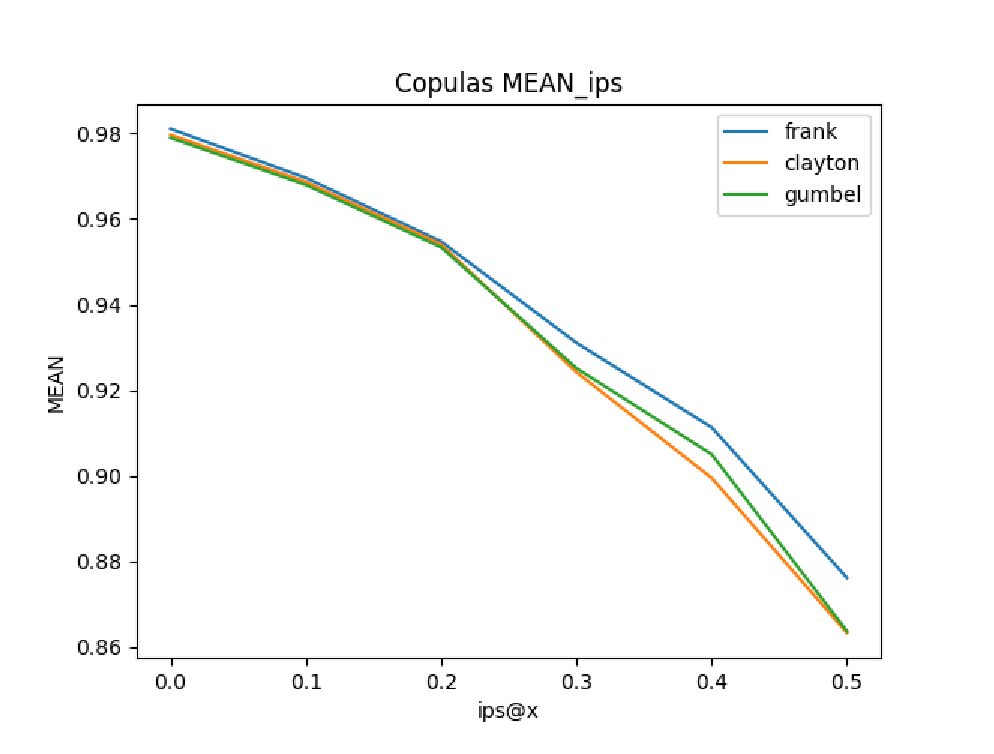
\includegraphics[width=7in]{source/copula_ip.eps}
  \vspace{1mm}
  \caption{コピュラのiP比較} %\vspace{-3mm}
  \label{fig:copula_ip}
  %\vspace{-0.4cm}
  \end{center} 
\end{figure}
\begin{figure}[H]
  \begin{center}
    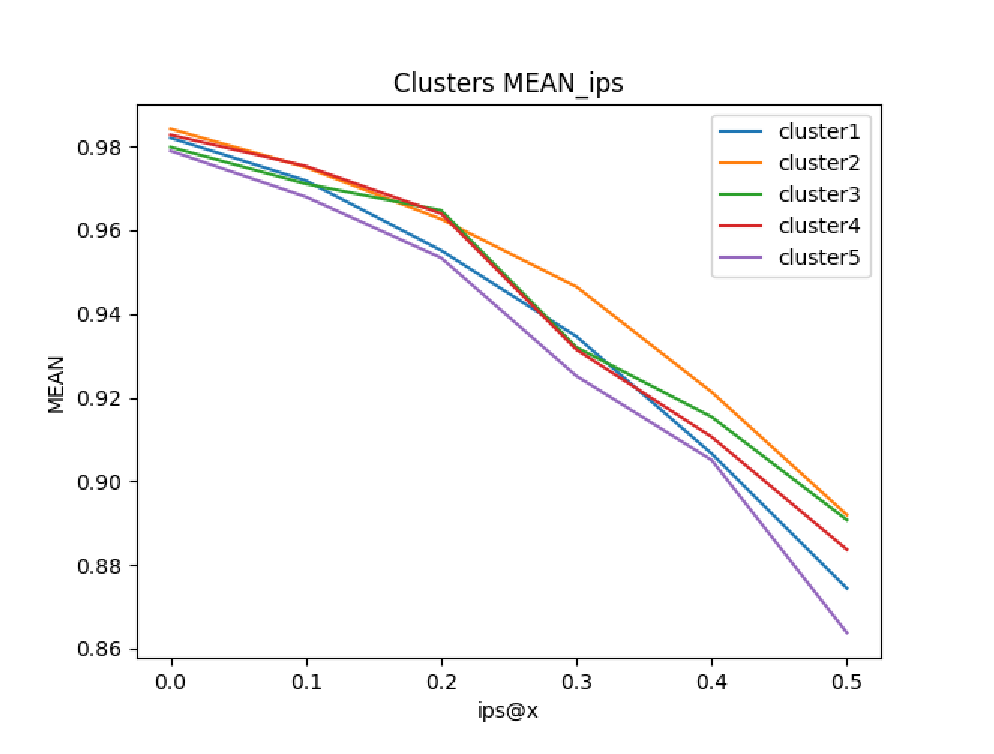
\includegraphics[width=7in]{source/cluster_ip.eps}
  \vspace{1mm}
  \caption{クラスタ数のiP比較} %\vspace{-3mm}
  \label{fig:cluster_ip}
  %\vspace{-0.4cm}
  \end{center} 
\end{figure}
\begin{figure}[H]
  \begin{center}
    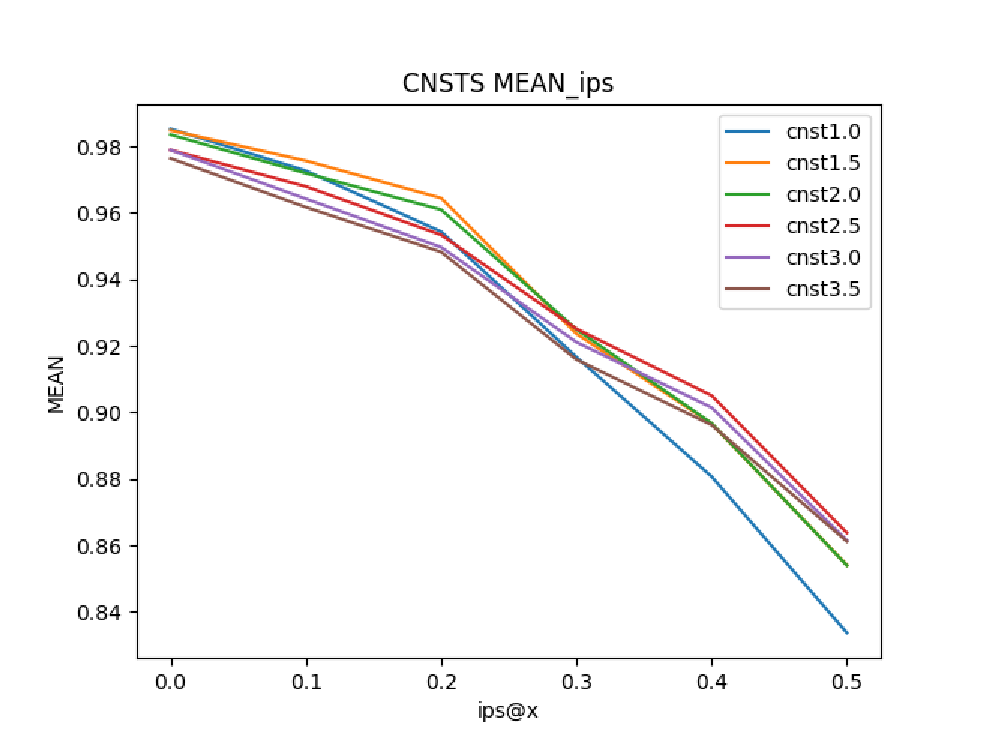
\includegraphics[width=7in]{source/cnst_ip.eps}
  \vspace{1mm}
  \caption{正定数cnstのiP比較} %\vspace{-3mm}
  \label{fig:cnst_ip}
  %\vspace{-0.4cm}
  \end{center} 
\end{figure}

%\chapter{Proof of Theorem 2}\label{appendix2}
%\chapter{定理2の証明}\label{appendix2}

% ----------------------------------------------------------------------
\end{document}
